\documentclass[10pt,oneside]{article}
\usepackage[T1]{fontenc}
\usepackage[utf8]{inputenc}
% \usepackage{lmodern}
%\usepackage[adobe-utopia,uppercase=upright,greeklowercase=upright]{mathdesign}
\usepackage[adobe-utopia]{mathdesign}
%\usepackage{minionpro}
% \usepackage{pifont}
% \usepackage{amssymb}
\usepackage{amsmath}
\usepackage[francais]{babel}
% \usepackage[francais]{varioref}
\usepackage[dvips]{graphicx}

\usepackage{framed}
\usepackage[normalem]{ulem}
\usepackage{fancyhdr}
\usepackage{titlesec}
\usepackage{vmargin}
\usepackage{longtable}

\usepackage{ifthen}


%\usepackage{epsfig}
\usepackage{subfig}

\usepackage{multirow}
\usepackage{multicol} % Portions de texte en colonnes
\usepackage{flafter}%floatants après la référence



\usepackage{color}
\usepackage{colortbl}


\definecolor{gris25}{gray}{0.75}
\definecolor{bleu}{RGB}{18,33,98}
\definecolor{bleuf}{RGB}{42,94,171}
\definecolor{bleuc}{RGB}{231,239,247}
\definecolor{rougef}{RGB}{185,18,27}
\definecolor{rougec}{RGB}{255,230,231}
\definecolor{vertf}{RGB}{103,126,82}
\definecolor{vertc}{RGB}{220,255,191}

\newenvironment{rem}[1][\hsize]%
{%
    \def\FrameCommand
    {%
\rotatebox{90}{\textit{\textsf{Remarque}}} 
        {\color{bleuf}\vrule width 3pt}%
        \hspace{0pt}%must no space.
        \fboxsep=\FrameSep\colorbox{bleuc}%
    }%
    \MakeFramed{\hsize#1\advance\hsize-\width\FrameRestore}%
}%
{\endMakeFramed}%


\newenvironment{savoir}[1][\hsize]%
{%
    \def\FrameCommand
    {%
\rotatebox{90}{\textit{\textsf{Savoir}}} 
        {\color{bleuf}\vrule width 3pt}%
        \hspace{0pt}%must no space.
        \fboxsep=\FrameSep\colorbox{bleuc}%
    }%
    \MakeFramed{\hsize#1\advance\hsize-\width\FrameRestore}%
}%
{\endMakeFramed}%

\newenvironment{prob}[1][\hsize]%
{%
    \def\FrameCommand%
    {%
\rotatebox{90}{\textit{\textsf{ Problématique}}} 
        {\color{rougef}\vrule width 3pt}%
        \hspace{0pt}%must no space.
        \fboxsep=\FrameSep\colorbox{rougec}%
    }%
    \MakeFramed{\hsize#1\advance\hsize-\width\FrameRestore}%
}%
{\endMakeFramed}%

\newenvironment{obj}[1][\hsize]%
{%
    \def\FrameCommand%
    {%
\rotatebox{90}{\textit{\textsf{ $\;$}}} 
        {\color{rougef}\vrule width 3pt}%
        \hspace{0pt}%must no space.
        \fboxsep=\FrameSep\colorbox{rougec}%
    }%
    \MakeFramed{\hsize#1\advance\hsize-\width\FrameRestore}%
}%
{\endMakeFramed}%

\newenvironment{defi}[1][\hsize]%
{%
    \def\FrameCommand%
    {%
\rotatebox{90}{\textit{\textsf{Définition\\}}} 
        {\color{bleuf}\vrule width 3pt}%
        \hspace{0pt}%must no space.
        \fboxsep=\FrameSep\colorbox{bleuc}%
    }%
    \MakeFramed{\hsize#1\advance\hsize-\width\FrameRestore}%
}%
{\endMakeFramed}%


\newenvironment{hypo}[1][\hsize]%
{%
    \def\FrameCommand%
    {%
\rotatebox{90}{\textit{\textsf{Hypothèse\\}}} 
        {\color{bleuf}\vrule width 3pt}%
        \hspace{0pt}%must no space.
        \fboxsep=\FrameSep\colorbox{bleuc}%
    }%
    \MakeFramed{\hsize#1\advance\hsize-\width\FrameRestore}%
}%
{\endMakeFramed}%


\newenvironment{prop}[1][\hsize]%
{%
    \def\FrameCommand%
    {%
\rotatebox{90}{\textit{\textsf{Propriété\\}}} 
        {\color{bleuf}\vrule width 3pt}%
        \hspace{0pt}%must no space.
        \fboxsep=\FrameSep\colorbox{bleuc}%
    }%
    \MakeFramed{\hsize#1\advance\hsize-\width\FrameRestore}%
}%
{\endMakeFramed}%

\newenvironment{props}[1][\hsize]%
{%
    \def\FrameCommand%
    {%
\rotatebox{90}{\textit{\textsf{Propriétés\\}}} 
        {\color{bleuf}\vrule width 3pt}%
        \hspace{0pt}%must no space.
        \fboxsep=\FrameSep\colorbox{bleuc}%
    }%
    \MakeFramed{\hsize#1\advance\hsize-\width\FrameRestore}%
}%
{\endMakeFramed}%

\newenvironment{exemple}[1][\hsize]%
{%
    \def\FrameCommand%
    {%
\rotatebox{90}{\textit{\textsf{Exemple\\}}} 
        {\color{vertf}\vrule width 3pt}%
        \hspace{0pt}%must no space.
        \fboxsep=\FrameSep\colorbox{vertc}%
    }%
    \MakeFramed{\hsize#1\advance\hsize-\width\FrameRestore}%
}%
{\endMakeFramed}%

\newenvironment{resultat}[1][\hsize]%
{%
    \def\FrameCommand%
    {%
\rotatebox{90}{\textit{\textsf{Résultat\\}}} 
        {\color{rougef}\vrule width 3pt}%
        \hspace{0pt}%must no space.
        \fboxsep=\FrameSep\colorbox{rougec}%
    }%
    \MakeFramed{\hsize#1\advance\hsize-\width\FrameRestore}%
}%
{\endMakeFramed}%

\newenvironment{methode}[1][\hsize]%
{%
    \def\FrameCommand%
    {%
\rotatebox{90}{\textit{\textsf{Méthode\\}}} 
        {\color{rougef}\vrule width 3pt}%
        \hspace{0pt}%must no space.
        \fboxsep=\FrameSep\colorbox{rougec}%
    }%
    \MakeFramed{\hsize#1\advance\hsize-\width\FrameRestore}%
}%
{\endMakeFramed}%

\newenvironment{theo}[1][\hsize]%
{%
    \def\FrameCommand%
    {%
\rotatebox{90}{\textit{\textsf{Théorème\\}}} 
        {\color{rougef}\vrule width 3pt}%
        \hspace{0pt}%must no space.
        \fboxsep=\FrameSep\colorbox{rougec}%
    }%
    \MakeFramed{\hsize#1\advance\hsize-\width\FrameRestore}%
}%
{\endMakeFramed}%

\newenvironment{warn}[1][\hsize]%
{%
    \def\FrameCommand%
    {%
\rotatebox{90}{\textit{\textsf{Attention\\}}} 
        {\color{rougef}\vrule width 3pt}%
        \hspace{0pt}%must no space.
        \fboxsep=\FrameSep\colorbox{rougec}%
    }%
    \MakeFramed{\hsize#1\advance\hsize-\width\FrameRestore}%
}%
{\endMakeFramed}%

% \usepackage{pstricks}
%\usepackage{minitoc}
% \setcounter{minitocdepth}{4}

\setcounter{tocdepth}{2}

% \mtcselectlanguage{french} 

%\usepackage{draftcopy}% "Brouillon"
% \usepackage{floatflt}
\usepackage{psfrag}
%\usepackage{listings} % Permet d'insérer du code de programmation
\renewcommand{\baselinestretch}{1.2}

% Changer la numérotation des figures :
% ------------------------------------
% \makeatletter
% \renewcommand{\thefigure}{\ifnum \c@section>\z@ \thesection.\fi
%  \@arabic\c@figure}
% \@addtoreset{figure}{section}
% \makeatother
 


%%%%%%%%%%%%
% Définition des vecteurs %
%%%%%%%%%%%%
 \newcommand{\vect}[1]{\overrightarrow{#1}}

%%%%%%%%%%%%
% Définition des torseusr %
%%%%%%%%%%%%

 \newcommand{\torseur}[1]{%
\left\{{#1}\right\}
}

\newcommand{\torseurcin}[3]{%
\left\{\mathcal{#1} \left(#2/#3 \right) \right\}
}

\newcommand{\torseurstat}[3]{%
\left\{\mathcal{#1} \left(#2\rightarrow #3 \right) \right\}
}

 \newcommand{\torseurc}[8]{%
%\left\{#1 \right\}=
\left\{
{#1}
\right\}
 = 
\left\{%
\begin{array}{cc}%
{#2} & {#5}\\%
{#3} & {#6}\\%
{#4} & {#7}\\%
\end{array}%
\right\}_{#8}%
}

 \newcommand{\torseurcol}[7]{
\left\{%
\begin{array}{cc}%
{#1} & {#4}\\%
{#2} & {#5}\\%
{#3} & {#6}\\%
\end{array}%
\right\}_{#7}%
}

 \newcommand{\torseurl}[3]{%
%\left\{\mathcal{#1}\right\}_{#2}=%
\left\{%
\begin{array}{l}%
{#1} \\%
{#2} %
\end{array}%
\right\}_{#3}%
}

 \newcommand{\vectv}[3]{%
\vect{V\left( {#1} \in {#2}/{#3}\right)}
}


\newcommand{\vectf}[2]{%
\vect{R\left( {#1} \rightarrow {#2}\right)}
}

\newcommand{\vectm}[3]{%
\vect{\mathcal{M}\left( {#1}, {#2} \rightarrow {#3}\right)}
}


 \newcommand{\vectg}[3]{%
\vect{\Gamma \left( {#1} \in {#2}/{#3}\right)}
}

 \newcommand{\vecto}[2]{%
\vect{\Omega\left( {#1}/{#2}\right)}
}
% }$$\left\{\mathcal{#1} \right\}_{#2} =%
% \left\{%
% \begin{array}{c}%
%  #3 \\%
%  #4 %
% \end{array}%
% \right\}_{#5}}

%  ------------------------------------------
% | Modification du formatage des sections : | 
%  ------------------------------------------

% Grands titres :
% ---------------

\newcommand{\titre}[1]{%
\begin{center}
      \bigskip
      \rule{\textwidth}{1pt}
      \par\vspace{0.1cm}
      
      \textbf{\large #1}
      \par\rule{\textwidth}{1pt}
    \end{center}
    \bigskip
  }

% Supprime le numéro du chapitre dans la numérotation des sections:
% -----------------------------------------------------------------
\makeatletter
\renewcommand{\thesection}{\@arabic\c@section}
\makeatother


% \titleformat{\chapter}[display]
% {\normalfont\Large\filcenter}
% {}
% {1pc}
% {\titlerule[1pt]
%   \vspace{1pc}%
%   \Huge}[\vspace{1ex}%
% \titlerule]


%%%% Chapitres Comme PY Pechard %%%%%%%%%
% numéro du chapitre
\DeclareFixedFont{\chapnumfont}{OT1}{phv}{b}{n}{80pt}
% pour le mot « Chapitre »
\DeclareFixedFont{\chapchapfont}{OT1}{phv}{m}{it}{40pt}
% pour le titre
\DeclareFixedFont{\chaptitfont}{T1}{phv}{b}{n}{25pt}

\definecolor{gris}{gray}{0.75}
\titleformat{\chapter}[display]%
	{\sffamily}%
	{\filleft\chapchapfont\color{gris}\chaptertitlename\
	\\
	\vspace{12pt}
	\chapnumfont\thechapter}%
	{16pt}%
	{\filleft\chaptitfont}%
	[\vspace{6pt}\titlerule\titlerule\titlerule]

%%%%  Fin Chapitres Comme PY Pechard %%%%%%%%%


% Section, subsection, subsubsection sans serifs :
% % ----------------------------------------------

% \makeatletter
% \renewcommand{\section}{\@startsection{section}{0}{0mm}%
% {\baselineskip}{.3\baselineskip}%
% {\normalfont\sffamily\Large\textbf}}%
% \makeatother

\makeatletter
\renewcommand{\@seccntformat}[1]{{\textcolor{bleu}{\csname
the#1\endcsname}\hspace{0.5em}}}
\makeatother

\makeatletter
\renewcommand{\section}{\@startsection{section}{1}{\z@}%
                       {-4ex \@plus -1ex \@minus -.4ex}%
                       {1ex \@plus.2ex }%
                       {\normalfont\Large\sffamily\bfseries}}%
\makeatother
 
\makeatletter
\renewcommand{\subsection}{\@startsection {subsection}{2}{\z@}
                          {-3ex \@plus -0.1ex \@minus -.4ex}%
                          {0.5ex \@plus.2ex }%
                          {\normalfont\large\sffamily\bfseries}}
\makeatother
 
\makeatletter
\renewcommand{\subsubsection}{\@startsection {subsubsection}{3}{\z@}
                          {-2ex \@plus -0.1ex \@minus -.2ex}%
                          {0.2ex \@plus.2ex }%
                          {\normalfont\large\sffamily\bfseries}}
\makeatother
 
\makeatletter             
\renewcommand{\paragraph}{\@startsection{paragraph}{4}{\z@}%
                                    {-2ex \@plus-.2ex \@minus .2ex}%
                                    {0.1ex}%               
{\normalfont\sffamily\bfseries}}
\makeatother
 
\makeatletter
\renewcommand{\subparagraph}{\@startsection{subparagraph}{5}{\z@}%
                                       {-2ex \@plus-.1ex \@minus .2ex}%
                                       {0.1ex}%
				    {\normalfont\normalsize\sffamily\bfseries}}
\makeatletter
% \makeatletter
% \renewcommand{\subsection}{\@startsection{subsection}{1}{2mm}%
% {\baselineskip}{.3\baselineskip}%
% {\normalfont\sffamily\large\textbf}}%
% \makeatother
% 
% \makeatletter
% \renewcommand{\subsubsection}{\@startsection{subsubsection}{2}{4mm}%
% {\baselineskip}{.15\baselineskip}%
% {\normalfont\sffamily\large\textbf}}%
% \makeatother
% 
% \makeatletter
% \renewcommand{\paragraph}{\@startsection{paragraph}{3}{6mm}%
% {\baselineskip}{.15\baselineskip}%
% {\normalfont\sffamily\large\textbf}}%
% \makeatother
 
\setcounter{secnumdepth}{4}


%  --------
% | Marges |
%  --------


% \setmarginsrb{2.5cm}{1.5cm}{2.5cm}{2cm}{1cm}{1cm}{1cm}{1cm}
\setmarginsrb{1.5cm}{1cm}{1cm}{1.5cm}{1cm}{1cm}{1cm}{1cm}

% Changer les marges localement :
% -----------------------------
\newenvironment{changemargin}[2]{\begin{list}{}{%
\setlength{\topsep}{0pt}%
\setlength{\leftmargin}{0pt}%
\setlength{\rightmargin}{0pt}%
\setlength{\listparindent}{\parindent}%
\setlength{\itemindent}{\parindent}%
\setlength{\parsep}{0pt plus 1pt}%
\addtolength{\leftmargin}{#1}%
\addtolength{\rightmargin}{#2}%
}\item }{\end{list}}



\usepackage{pst-solides3d}
\usepackage{titletoc}
\titlecontents{chapter}[+3pc]
  {\addvspace{10pt}\sffamily\bfseries}
{\contentslabel[{\pscirclebox[fillstyle=solid,fillcolor=gray!25,
linecolor=gray!25,framesep=4pt]{\textcolor{white}{\thecontentslabel}}}]{2.5pc}}
  {}
  {\dotfill \normalfont\thecontentspage\ }

\titlecontents{section}[3pc]
  {\addvspace{2pt}\sffamily}
  {\contentslabel[\thecontentslabel]{1.8pc}}
  {}
  {\dotfill \normalfont\thecontentspage\ }

\titlecontents{subsection}[5pc]
  {\addvspace{2pt}\sffamily}
  {\contentslabel[\thecontentslabel]{1.8pc}}
  {}
  {\dotfill \normalfont\thecontentspage\ }

\titlecontents{subsubsection}[8pc]
  {\addvspace{2pt}\sffamily}
  {\contentslabel[\thecontentslabel]{3pc}}
  {}
  {\dotfill \normalfont\thecontentspage\ }
%{\;\titlerule\;\normalfont\thecontentspage\ }

\titlecontents{paragraph}[9pc]
  {\addvspace{2pt}\sffamily}
  {\contentslabel[\thecontentslabel]{3.5pc}}
  {}
  {\dotfill \normalfont\thecontentspage\ }



%% !TEX encoding = UTF8
%
%\documentclass[a4paper, 11 pt]{article}
%
%\usepackage[francais, frenchb]{babel}
%\usepackage[T1]{fontenc}
%\usepackage[utf8]{inputenc}
%\usepackage{url}
%\usepackage{multicol}
%\usepackage{graphicx}
%\usepackage{xargs}
%\usepackage[usenames,svgnames,dvipsnames]{xcolor}
%\usepackage[leqno, fleqn]{amsmath}
%\usepackage{amssymb}
%\usepackage{mathtools}
%\usepackage{wrapfig}
%\usepackage{enumerate}
%\usepackage{longtable}
%\usepackage{tabularx}
\usepackage{tikz}
%\usetikzlibrary{shapes}
%\usetikzlibrary{calc}
%\usepackage{enumitem}
%\usepackage{fancyhdr}
%\usepackage{caption}
%\usepackage{subcaption}
%\usepackage{ifthen}
%\usepackage{calc}
%\usepackage{fp}
%\usepackage{multido}
%\usepackage{lscape}
%\usepackage{titling}
%\usepackage{cancel}
%\usepackage{geometry}
%\usepackage{float}
%\usepackage{palatino}


\definecolor{bleuppt}{RGB}{0,112,192}

%Commande pour tracer des figures planes: \figureplane
\newcommand\figureplane[9]{
\begin{tikzpicture}[scale=#9]
\draw[thick,->,#7] (0,0) -- (0:1) node[anchor=north west]{$\vec{#1}$};
\draw[thick,->,#7] (0,0) -- (90:1) node[anchor=north east]{$\vec{#3}$}; 
\draw[thick,->,#8] (0,0) -- (20:1) node[anchor=south east]{$\vec{#2}$}; 
\draw[thick,->,#8] (0,0) -- (110:1) node[anchor=north east]{$\vec{#4}$}; 
\fill[white] (0,0) circle (0.05);
\draw[thick,#7] (0,0) circle (0.05);
\fill[#7] (0,0) circle (0.01);
\draw (-0.05,0) node[anchor=north east] {$\vec{#5}$};
\draw[thick,->] (0.4,0) arc (0:20:0.4);
\draw[thick,->] (0,0.4) arc (90:110:0.4);
\draw (0.4,0.08) node[anchor=west] {$#6$};
\draw (-0.08,0.4) node[anchor=south] {$#6$};
\end{tikzpicture}
}

%couleurs des figures planes pour ne pas dépasser neuf arguments
\newcommand\couleursfigureplane[2]{%
    \def\premierecouleur{#1}%
    \def\deuxiemecouleur{#2}%
}

%Commande pour tracer des figures planes avec reperes: \figureplanerep
\newcommand\figureplanerep[9]{
\begin{tikzpicture}[scale=#9]
\draw[thick,->,\premierecouleur ] (0,0) -- (0:1) node[anchor=north west]{$\vec{#1}$};
\draw[thick,->,\premierecouleur ] (0,0) -- (90:1) node[anchor=north east]{$\vec{#3}$}; 
\draw[thick,->,\deuxiemecouleur ] (0,0) -- (20:1) node[anchor=south east]{$\vec{#2}$}; 
\draw[thick,->,\deuxiemecouleur ] (0,0) -- (110:1) node[anchor=north east]{$\vec{#4}$}; 
\fill[white] (0,0) circle (0.05);
\draw[thick,\premierecouleur] (0,0) circle (0.05);
\fill[\premierecouleur] (0,0) circle (0.01);
\draw[\premierecouleur] (-0.05,0) node[anchor=north east] {$\vec{#5}$};
\draw[thick,->] (0.4,0) arc (0:20:0.4);
\draw[thick,->] (0,0.4) arc (90:110:0.4);
\draw[thick,\premierecouleur] (0:0.5) arc (180:360:0.15) ;
\draw[\premierecouleur] (0.65,-0.07) node{\ensuremath{#7}};
\draw[thick,\deuxiemecouleur] (20:0.8) arc (20:200:0.15);
\draw[\deuxiemecouleur] (0.59,0.29) node{\ensuremath{#8}};
\draw (0.4,0.08) node[anchor=west] {$#6$};
\draw (-0.08,0.4) node[anchor=south] {$#6$};
\end{tikzpicture}
}

%\begin{document}
%
%Pour tracer une figure plane sans les repères de bases : les couleurs sont indiquées directement dans la commande.
%\begin{verbatim}
%\figureplane{x_0}{x_1}{y_0}{y_1}{z_0}{\theta}{blue}{red}{4}
%\end{verbatim}
%\figureplane{x_0}{x_1}{y_0}{y_1}{z_0}{\theta}{blue}{red}{4}
%\vspace{3cm}
%
%Pour tracer une figure plane avec les repères de bases : les couleurs sont indiquées avant la commande pour ne pas dépasser neuf arguments.
%\begin{verbatim}
%\couleursfigureplane{blue}{red}
%\figureplanerep{x_0}{x_1}{y_0}{y_1}{z_0}{\theta}{0}{1}{4}
%\end{verbatim}
%\couleursfigureplane{blue}{red}
%\figureplanerep{x_0}{x_1}{y_0}{y_1}{z_0}{\theta}{0}{1}{4}
%
%
%\end{document}
%
%
%
%
%
%


%Si le boolen xp est vrai : compilation pour xabi
%Sinon compilation Damien
\newboolean{xp}
\setboolean{xp}{true}

\newboolean{prof}
\setboolean{prof}{true}

\def\xxtitre{\ifthenelse{\boolean{xp}}{
CI 3 -- CIN : Étude du comportement cinématique des systèmes}{
}}

\def\xxsoustitre{\ifthenelse{\boolean{xp}}{
Chapitre 2 -- Géométrie dans l'espace}{
}}


\def\xxauteur{\ifthenelse{\boolean{xp}}{
\noindent 2013 -- 2014 \\
Xavier \textsc{Pessoles}}{
}}


\def\xxpied{\ifthenelse{\boolean{xp}}{
CI 3 : CIN -- Cours \\
Ch 2 : Géométrie dans l'espace -- \ifthenelse{\boolean{prof}}{P}{E}%
}{
}}

\usepackage[%
    pdftitle={CIN : Géométrie dans l'espace},
    pdfauthor={Xavier Pessoles},
    colorlinks=true,
    linkcolor=blue,
    citecolor=magenta]{hyperref}


\newcommand{\Det}{\mathrm{Det}\hspace{.2mm}}
\usepackage{pifont}
\sloppy
\hyphenpenalty 10000


\begin{document}






% \makeatletter \let\ps@plain\ps@empty \makeatother
%% DEBUT DU DOCUMENT
%% =================




%------------- En tetes et Pieds de Pages ------------


\pagestyle{fancy}
\ifthenelse{\boolean{xp}}{%
\renewcommand{\headrulewidth}{0pt}}{%
\renewcommand{\headrulewidth}{0.2pt}} %pour mettre le trait en haut
%\renewcommand{\headrulewidth}{0.2pt}

\fancyhead{}
\fancyhead[L]{%
\ifthenelse{\boolean{xp}}{%
\noindent\begin{minipage}[c]{2.6cm}%

\includegraphics[width=2cm]{png/logo_ptsi.png}%
\end{minipage}%
}{%
\footnotesize{\textit{\textsf{Lycée François Premier}}}
}}

\ifthenelse{\boolean{xp}}{%
\fancyhead[C]{\rule{12cm}{.5pt}}}{
}


\fancyhead[R]{%
\noindent\begin{minipage}[c]{3cm}
\begin{flushright}
\footnotesize{\textit{\textsf{Sciences Industrielles \\ de l'ingénieur}}}%
\end{flushright}
\end{minipage}
}


\ifthenelse{\boolean{xp}}{%
\fancyhead[C]{\rule{12cm}{.5pt}}}{
}

\renewcommand{\footrulewidth}{0.2pt}

\fancyfoot[C]{\footnotesize{\bfseries \thepage}}
\fancyfoot[L]{%
\begin{minipage}[c]{.2\linewidth}
\noindent\footnotesize{{\xxauteur}}
\end{minipage}
\ifthenelse{\boolean{xp}}{}{%
\begin{minipage}[c]{.15\linewidth}

\includegraphics[width=2cm]{png/logoCC.png}
\end{minipage}}
}


\fancyfoot[R]{\footnotesize{\xxpied}}



\begin{center}
 \huge\textsc{\xxtitre}
\end{center}

\begin{center}
 \LARGE\textsc{\xxsoustitre}
\end{center}




\begin{center}
\begin{tabular}{ccccc}
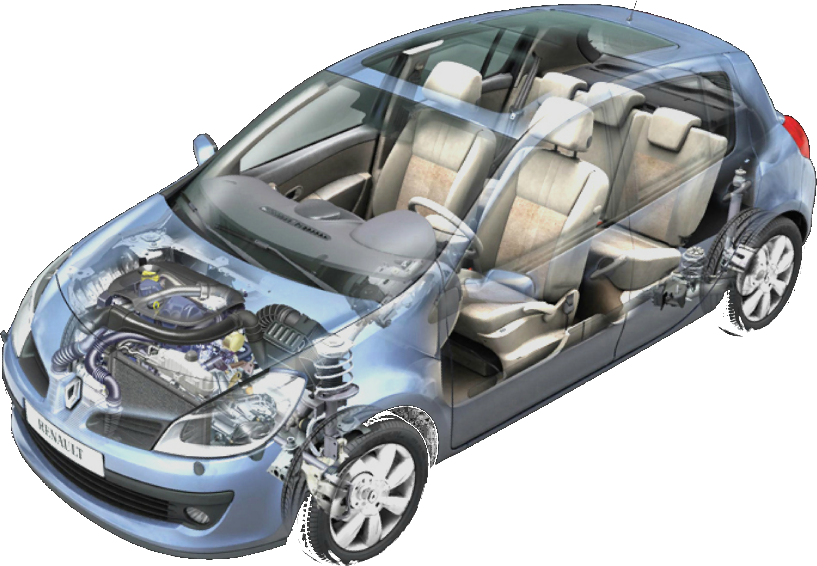
\includegraphics[width=4cm]{png/voiture} &&
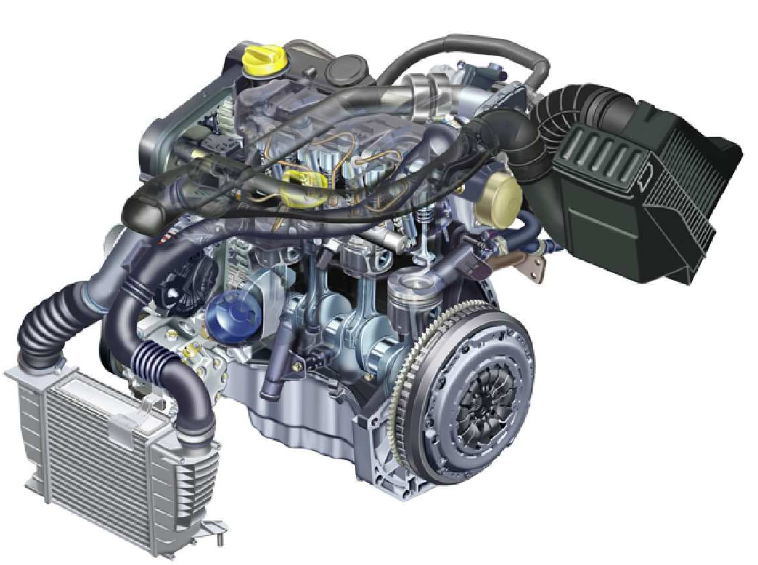
\includegraphics[height=4cm]{png/moteur} && 
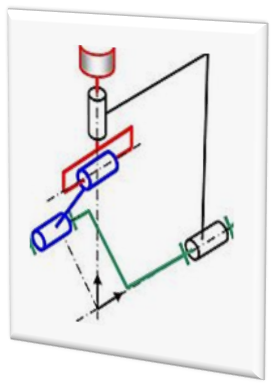
\includegraphics[height=4cm]{png/ex_schema}\\
\textit{Effeuillage d'un Renault Clio \cite{cite1}} &&
\textit{Moteur 1.5 dCi K9K 105 ch \cite{cite1}} &&
\textit{Modélisation par schéma cinématique\cite{cite2}}\\
\end{tabular}
\end{center}

\vspace{.2cm}

%
%\begin{obj}
%\textbf{Problématique :}
%\begin{itemize}
%\item M
%\end{itemize}
%\end{obj}

\begin{savoir}
\textbf{Savoirs :}
\begin{itemize}
\item Manipuler des vecteurs, les repères et les différents systèmes de coordonnées
\item Calculer un produit scalaire
\item Calculer un produit vectoriel
\item Calculer un produit mixte
\end{itemize}
\end{savoir}

\setlength{\parskip}{0ex plus 0.2ex minus 0ex}
 \renewcommand{\contentsname}{}
 \renewcommand{\baselinestretch}{1}

% \vspace{1cm}
\textit{Les sections 1, 2, 3 et 4 sont lagement inspirées du cours de géométrie de P. Soleillant \cite{PS,DP}.}

\textit{Ce document est en évolution permanente. Merci de signaler toutes
erreurs ou coquilles.}

\tableofcontents

 \renewcommand{\baselinestretch}{1.2}
\setlength{\parskip}{2ex plus 0.5ex minus 0.2ex}



\section{Vecteurs}
On postule l'existence d'un ensemble, appelé plan euclidien, et noté $\mathcal{P}$. Ses éléments sont appelés points.
\subsection{Définitions}
\begin{defi}
\textbf{Vecteurs}

Soit $(A;B)$ un couple\footnotemark[1] de points du plan : ce couple définit :
\begin{itemize}
\item une direction (celle de la droite $(AB)$);
\item un sens (de $A$ vers $B$);
\item une longueur (la longueur $AB$).
\end{itemize}

On associe à un tel couple un objet appelé \textbf{vecteur}, noté $\vect{AB}$.
\end{defi}

\footnotetext[1]{Attention à l'ordre : $A$ \textbf{puis} $B$.}

\begin{rem}
\textbf{Bipoints équipollents}

Le tracé de la <<flèche>> $(A,B)$ est appelé bipoint. Deux bipoints sont équipollents s'ils ont même direction, même sens et même norme. 
\end{rem}

\subsection{Règles de calcul}
\begin{minipage}[c]{.7\linewidth}
\begin{propo}
\textbf{Égalité de deux vecteurs}

Deux vecteurs $\vect{AB}$ et $\vect{CD}$  sont égaux lorsqu'ils ont même direction, même sens et même longueur. Les
couples de points $(A;B)$ et $(C;D)$ définissent alors un même vecteur. On dit parfois que $\vect{AB}$ est un représentant du vecteur $\vect{v}$.

Le vecteur $\vect{AB}$ est dit nul lorsque $A = B$. Le vecteur
nul est noté $\vect{0}$.

Étant donnés un point $O$ et un vecteur $\vect{v} = \vect{AB}$, il existe un unique point $M$ du plan tel que $\vect{v} = \vect{OM}$.

\end{propo}

\end{minipage}\hfill
\begin{minipage}[c]{.28\linewidth}
\begin{center}
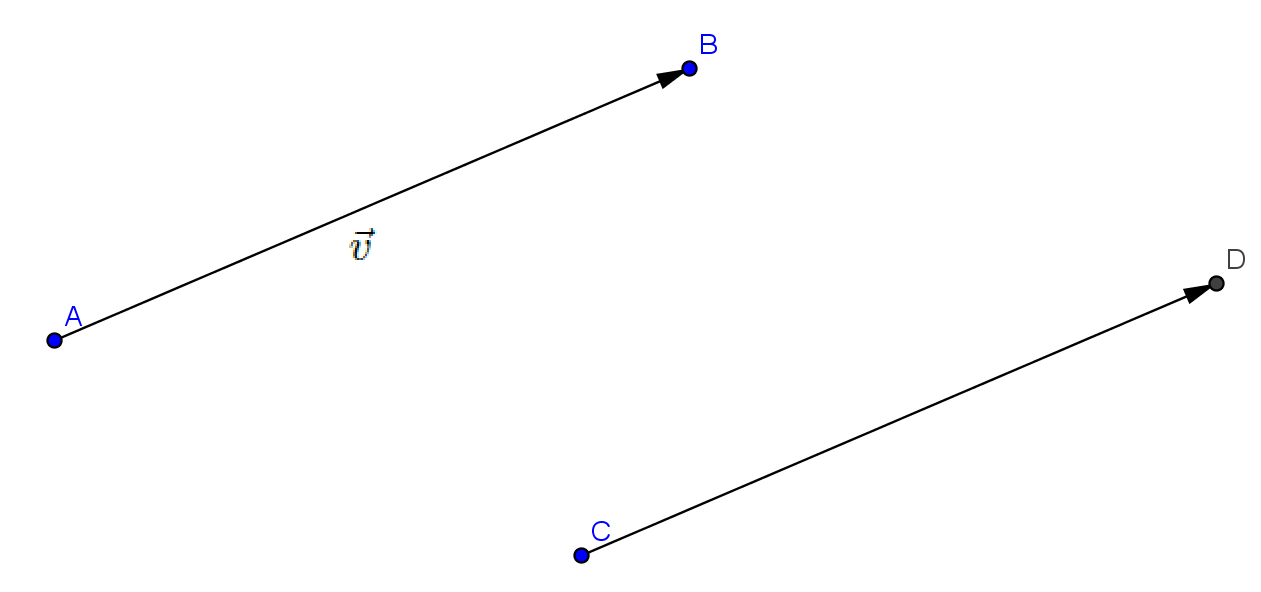
\includegraphics[width=.95\textwidth]{png/vecteur}
\end{center}
\end{minipage}

\begin{minipage}[c]{.7\linewidth}
\begin{propo}
\textbf{Produit par un réel}

Soient $A$ et $B$ deux points distincts et $\lambda\in \mathbb{R}$. On définit le vecteur $\lambda\cdot \vect{AB}$ comme le vecteur $\vect{AC}$ où $C$ est le point de la droite $(AB)$ qui vérifie 
$$
\dfrac{\overline{AC}}{\overline{AB}} = \lambda
$$
 où $\overline{AC}$ et $\overline{AB}$ sont les mesures algébriques respectives des couples $(A,C)$ et $(A,B)$ dans un repère arbitraire de la droite $(AB)$.

Dans le cas du vecteur nul, on pose $\lambda \cdot \vect{0} =\vect{0}$.
\end{propo}
\end{minipage}\hfill
\begin{minipage}[c]{.28\linewidth}
\begin{center}
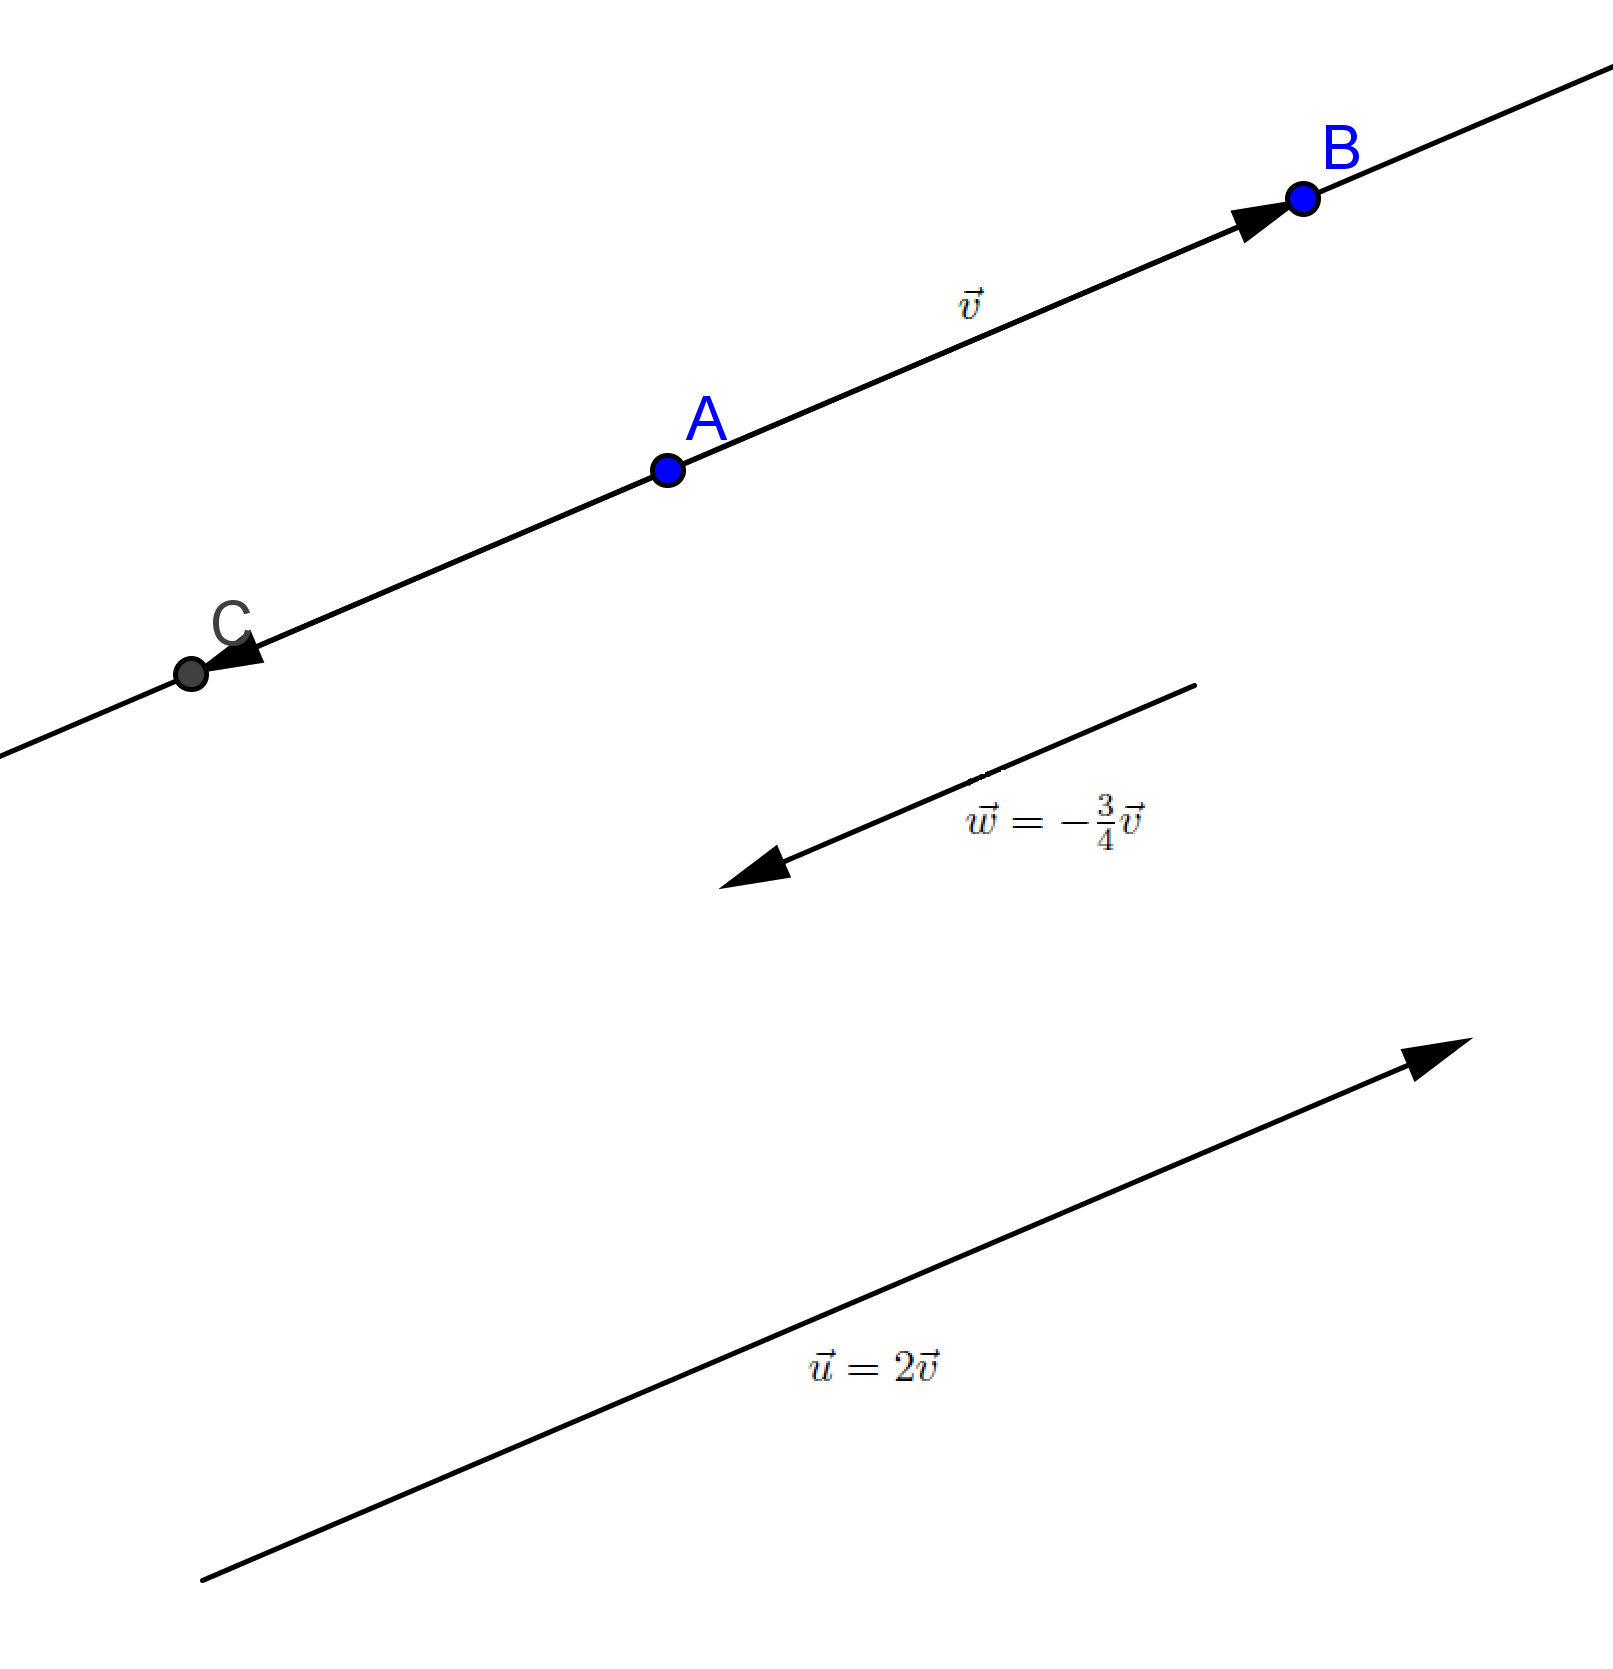
\includegraphics[width=.95\textwidth]{png/produit_vecteur}
\end{center}
\end{minipage}



\begin{rem}
\textit{Mesure algébrique}


Soient une droite $\mathcal{D}$, un point origine $O$ sur $\mathcal{D}$ et un point $I$ sur $\mathcal{D}$ tel que $OI=1$. 

Soient $M$ et $N$ deux points de $\mathcal{D}$ d'abscisses respectives $x_M$ et $x_N$. On appelle mesure algébrique du couple $(M,N)$ (dans cet ordre) dans le repère $(O,I)$, et on note $\overline{MN}$ le réel tel que 
$$
\overline{MN} = x_N - x_M
$$
\end{rem}

\begin{minipage}[c]{.7\linewidth}
\begin{propo}
\textbf{Addition de deux vecteurs}

Soient $\vect{v}$ et $\vect{w}$ deux vecteurs. On peut les représenter sous la forme $\vect{v}=\vect{OM}$ et $\vect{w}=\vect{ON}$. On définit $\vect{v}+\vect{w}$ comme le vecteur $\vect{OP}$ tel que le quadrilatère $OMPN$ soit un parallélogramme. Ce vecteur $\vect{v}+\vect{w}$ ne dépend pas du choix du point $O$. 

Une conséquence essentielle de cette définition de l'addition de vecteurs est la \textbf{relation de Chasles} $\vect{AC}=\vect{AB}+\vect{BC}$. 
\end{propo}
\end{minipage}\hfill
\begin{minipage}[c]{.28\linewidth}
\begin{center}
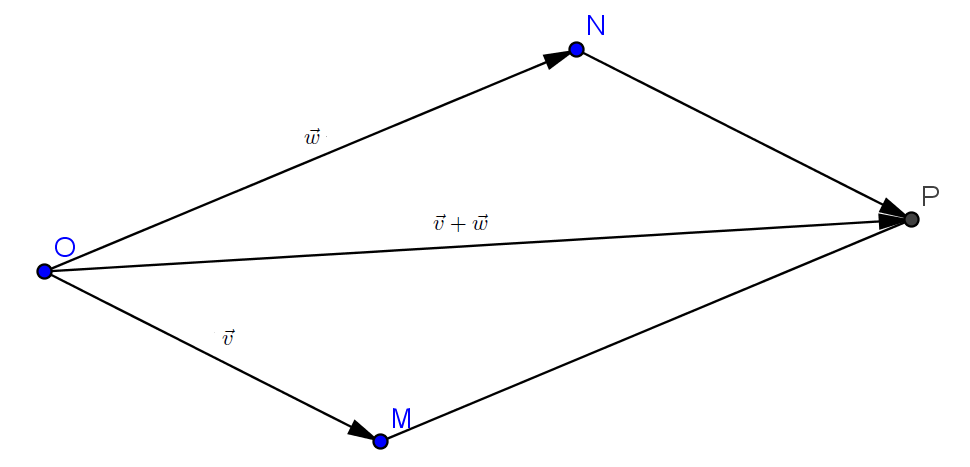
\includegraphics[width=.95\textwidth]{png/somme_vecteur}
\end{center}
\end{minipage}


\begin{propo}
\textbf{Norme d'un vecteur}

On appelle la norme du vecteur $\vect{v}=\vect{AB}$ la longueur du segment $[AB]$. Elle ne dépend pas du représentant choisi, c'est-à-dire que si $C$ et $D$ sont des points du plan vérifiant aussi $\vect{v}=\vect{CD}$, alors on a : $AB=CD$. 
\end{propo}

%%%%%%%%%%%%%%%%%%%%%%%%%%%%


\section{Modes de repérage dans l'espace}

\subsection{Repère(s) cartésien(s) de l'espace}

\begin{defi}
\textbf{Repère cartésien}

On appelle repère cartésien de $\mathcal{E}$ la donnée d'un point $O$ du plan, et de trois vecteurs $\vect{i}$, $\vect{j}$ et $\vect{k}$ non coplanaires.

Le point $O$ est appelé origine du repère, le triplet de vecteurs $(\vect{i}, \vect{j}, \vect{k})$ est appelé base du repère.
\end{defi}

\begin{rem}

\begin{enumerate}
\item Pour tout point $M$ de l'espace, il existe un unique triplet de réels $(x,y,z)$ vérifiant :
$$\overrightarrow{OM}=x\vect{i}+y\vect{j}+z\vect{k}.$$

Le réel $x$ est appelé abscisse de $M$ dans le repère $(O,\vect{i}, \vect{j}, \vect{k})$, le réel $y$ est appelé ordonnée de $M$ dans le repère $(O,\vect{i}, \vect{j}, \vect{k})$ et le réel $z$ est appelé cote de $M$ dans le repère $(O, \vect{i}, \vect{j}, \vect{k})$. Enfin, le triplet $(x,y,z)$ est appelé triplet de coordonnées (cartésiennes) de $M$ dans le repère $(O,\vect{i}, \vect{j}, \vect{k})$.
\item On définit, de même, les coordonnées d'un vecteur $\vect{u}$ de l'espace, dans la base $(\vect{i}, \vect{j}, \vect{k})$, comme l'unique triplet de réels $(x,y,z)$ vérifiant $\vect{u}=x\vect{i}+y\vect{j}+z\vect{k}$.
\item Si, dans la base $(\vect{i}, \vect{j}, \vect{k})$, $\vect{u}$ a pour coordonnées $(x,y,z)$ et $\vec v$ a pour coordonnées $(x',y',z')$, alors $\vect{u}+\vec v$ a pour coordonnées $(x+x',y+y',z+z')$, et si $\lambda \in \mathbb{R}$, les coordonnées de $\lambda \vect{u}$ sont $(\lambda x,\lambda y, \lambda z)$.
\item Étant donnés deux points $A$ et $B$ de l'espace, de coordonnées respectivement $(x_A,y_A,z_A)$ et $(x_B,y_B,z_B)$ dans $(O,\vect{i}, \vect{j},\vect{k})$, les coordonnées de $\overrightarrow{AB}$ dans $(\vect{i}, \vect{j}, \vect{k})$ sont $(x_B-x_A,y_B-y_A,z_B-z_A)$ (pour s'en assurer, il suffit d'écrire $\overrightarrow{AB}=\overrightarrow{OB}-\overrightarrow{OA}$).
%\item De même, on peut exprimer simplement les coordonnées du barycentre d'un système de points pondérés. En effet, si
%$\lambda_1$, $\lambda_2$, ... , $\lambda_n$ sont $n$ réels tels que $\lambda_1+\lambda_2+\cdots + \lambda_n \neq 0$
%et $A_1$, $A_2$, ... , $A_n$ sont $n$ points de l'espace, le barycentre $G$ de $\{(A_1,\lambda_1),(A_2,\lambda_2), \cdots , (A_n,\lambda_n)\}$
%vérifie :
%$$\lambda_1 \overrightarrow{OA_1}+\lambda_2 \overrightarrow{OA_2}+\cdots +\lambda_n \overrightarrow{OA_n}=(\lambda_1+\lambda_2+\cdots + \lambda_n) \overrightarrow{OG}.$$
%On en déduit aisément que les coordonnées de $G$ sont :
%$$\left(\frac{\lambda_1x_1+\lambda_2x_2+ \cdots+ \lambda_nx_n}{\lambda_1+\lambda_2+\cdots +\lambda_n},\frac{\lambda_1y_1+\lambda_2y_2+ \cdots +\lambda_ny_n}{\lambda_1+\lambda_2+\cdots +\lambda_n},
%\frac{\lambda_1z_1+\lambda_2z_2+ \cdots +\lambda_nz_n}{\lambda_1+\lambda_2+\cdots +\lambda_n}\right),$$
%où, pour tout $i \in [|1,n|]$, $(x_i,y_i,z_i)$ sont les coordonnées de $A_i$ dans le repère $(O, \vect{i}, \vect{j}, \vect{k})$.
%\item Par définition, les coordonnées d'un point ou d'un vecteur de l'espace dépendent du repère cartésien choisi.

%Par exemple, si l'on considère un repère cartésien $(O, \vect{i}, \vect{j}, \vect{k})$ de l'espace, et le point $\Omega$ ayant pour coordonnées
%$(a,b,c)$ dans $(O, \vect{i}, \vect{j}, \vect{k})$, alors $(\Omega, \vect{i}, \vect{j}, \vect{k})$ est un autre repère cartésien de l'espace.

%Tout point $M$ de l'espace ayant pour coordonnées $(x,y,z)$ dans $(O, \vect{i}, \vect{j}, \vect{k})$ a pour coordonnées $(x-a,y-b,z-c)$ dans le repère
%$(\Omega, \vect{i}, \vect{j}, \vect{k})$.

%En outre, $(\Omega, \vect{k}, \vect{i}, \vect{j})$ est aussi un repère cartésien de l'espace, et tout point $M$ du plan ayant pour coordonnées $(x,y,z)$ dans $(O, \vect{i}, \vect{j}, \vect{k})$ a pour coordonnées $(z-c,x-a,y-b)$ dans le repère $(\Omega, \vect{k}, \vect{i},\vect{j})$.
\item L'intérêt de munir l'espace euclidien d'un repère cartésien réside dans le fait qu'à chaque point (resp. à chaque vecteur) de l'espace correspond un unique triplet de réels -- et réciproquement.
Ainsi, on peut exprimer toutes les propriétés des points et des vecteurs que l'on considère par des relations algébriques entre
leurs coordonnées... qui ne sont "que" des triplets de réels !
\end{enumerate}

\end{rem}

\begin{exemple}
\textit{Trajectoire en coordonnées cartésiennes}

\begin{minipage}[c]{.47\linewidth}
\begin{center}
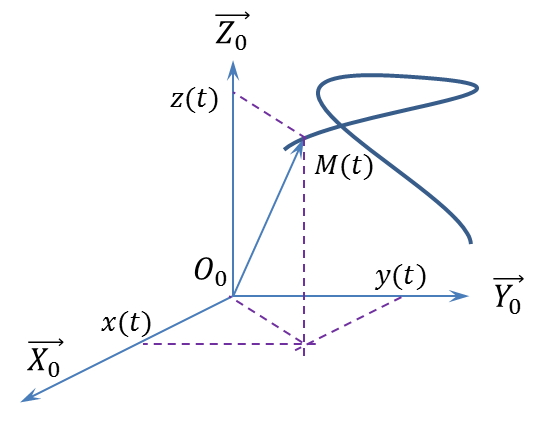
\includegraphics[width=.8\textwidth]{png/coord_cartesiennes}
\end{center}
\end{minipage}\hfill
\begin{minipage}[c]{.47\linewidth}
Le point $M$ suit une trajectoire dans le repère $\mathcal{R}_0=\left(O_0, \vect{X_0},\vect{Y_0},\vect{Z_0}\right)$
$$
\vect{OM(t)}=x(t)\vect{X_0}+y(t)\vect{Y_0}+z(t)\vect{Z_0}
=\left[
\begin{array}{l}
x(t) \\
y(t) \\
z(t) 
\end{array}
\right]_{\mathcal{R}_0}
$$
\end{minipage}
\end{exemple}

\begin{defi}
\textbf{Repère orthogonal, orthonormal}

Soit $(O,\vect{i}, \vect{j}, \vect{k})$ un repère cartésien de l'espace.

On dit que $(O,\vect{i}, \vect{j}, \vect{k})$ (respectivement la base $(\vect{i}, \vect{j}, \vect{k})$) est un repère (respectivement une base) orthogonal(e) lorsque les vecteurs $\vect{i}$, $\vect{j}$ et $\vect{k}$ sont deux à deux orthogonaux.

Lorsque, en outre, $||\vect{i}||=||\vect{j}||=||\vect{k}||=1$, le repère $(O, \vect{i}, \vect{j}, \vect{k})$ (respectivement la base) $(\vect{i}, \vect{j}, \vect{k})$) est dit(e) orthonormé(e).
\end{defi}


\begin{rem}

On verra que les propriétés liées à l'orthogonalité, aux distances et aux angles s'expriment plus simplement dans un repère orthonormal que dans un repère plus <<quelconque>>. Ainsi, on se placera souvent dans un repère orthonormé.
\end{rem}

\subsection{Orientation de l'espace, repères (orthonormés) directs}

Soient $O$ un point de l'espace et $\vect{i}$ et $\vect{j}$ deux vecteurs orthogonaux et de norme 1. Il existe un unique plan $\mathcal{P}$ contenant $O$, $\vect{i}$ et $\vect{j}$. On voit alors que, si l'on cherche un vecteur $\vect{k}$ de sorte que $(O, \vect{i}, \vect{j}, \vect{k})$ soit un repère orthonormé de l'espace, sa direction est imposée : le vecteur $\vect{k}$ doit être orthogonal au plan $\mathscr P$. Reste à préciser son sens : pour cela, on a deux possibilités. On peut, par exemple, choisir $\vect{k}$ de sorte que la succession $(\vect{i}, \vect{j}, \vect{k})$ soit dans la même configuration spatiale que le triplet (pouce, indexe, majeur)\footnote{Le pouce et l'index étant totalement "déployés", tandis que le majeur est levé à la verticale de la paume.} de la main droite (dans cet ordre !). Dans ce cas, on dit que le repère $(O, \vect{i}, \vect{j}, \vect{k})$ est \emph{direct}. Dans le cas contraire, le repère est dit \emph{indirect} ou \emph{rétrograde}. Par ce choix (arbitraire) de classer les repères orthonormés de l'espace en deux catégories (directs ou indirects), on dit qu'on a \emph{orienté} l'espace $\mathcal{E}$.

%Il n'existe aucun crit�re math�matique pour privil�gier une orientation plut�t qu'une autre : ce choix ne peut �tre qu'arbitraire. En g�n�ral, on convient de dire que le rep�re $(O, \vect{i}, \vect{j}, \vect{k})$ est direct lorsque... Ces conventions sont souvent utilis�es en physique (�lectromagn�tisme) et en chimie(mol�cules chirales).

\begin{rem}

\begin{enumerate}
\item On peut également définir la notion de repère direct sans que la base associée soit nécessairement orthonormée : un repère cartésien $(O, \vect{i}, \vect{j}, \vect{k})$ est dit direct lorsque $(\vect{i}, \vect{j}, \vect{k})$ est dans la même configuration spatiale que le triplet (pouce, indexe, majeur)... qui peuvent être disposés sans former des directions nécessairement perpendiculaires les unes aux autres. Un repère est dit rétrograde lorsqu'il n'est pas direct.

Dans le premier cas, on dit que le triplet de vecteurs $(\vect{i}, \vect{j}, \vect{k})$ est une \emph{base directe}, et dans le second, que c'est une \emph{base indirecte} ou \emph{rétrograde}.
\item Signalons que l'orientation de l'espace n'induit pas d'orientation particulière d'un plan de cet espace. Pour orienter un plan $\mathscr P$, il suffit d'orienter une droite $\mathscr D$ orthogonale à $\mathscr P$, en choisissant un vecteur $\vect{k}$ unitaire de $\mathscr D$ (il y a deux possibilités) : une base orthonormale $(\vect{i}, \vect{j})$ de $\mathscr P$ sera dite directe pour l'orientation définie par $\vect{k}$ lorsque la base $(\vect{i}, \vect{j}, \vect{k})$ est directe dans l'espace. On dit alors qu'on a orienté le plan $\mathscr P$ par le vecteur normal $\vect{k}$.\\
\end{enumerate}

\end{rem}
%\subsection{Changement de rep�re}

\subsection{Exemple}

Considérons le cas d'un micromoteur de modélisme modélisé par son schéma cinématique minimal.


\begin{center}
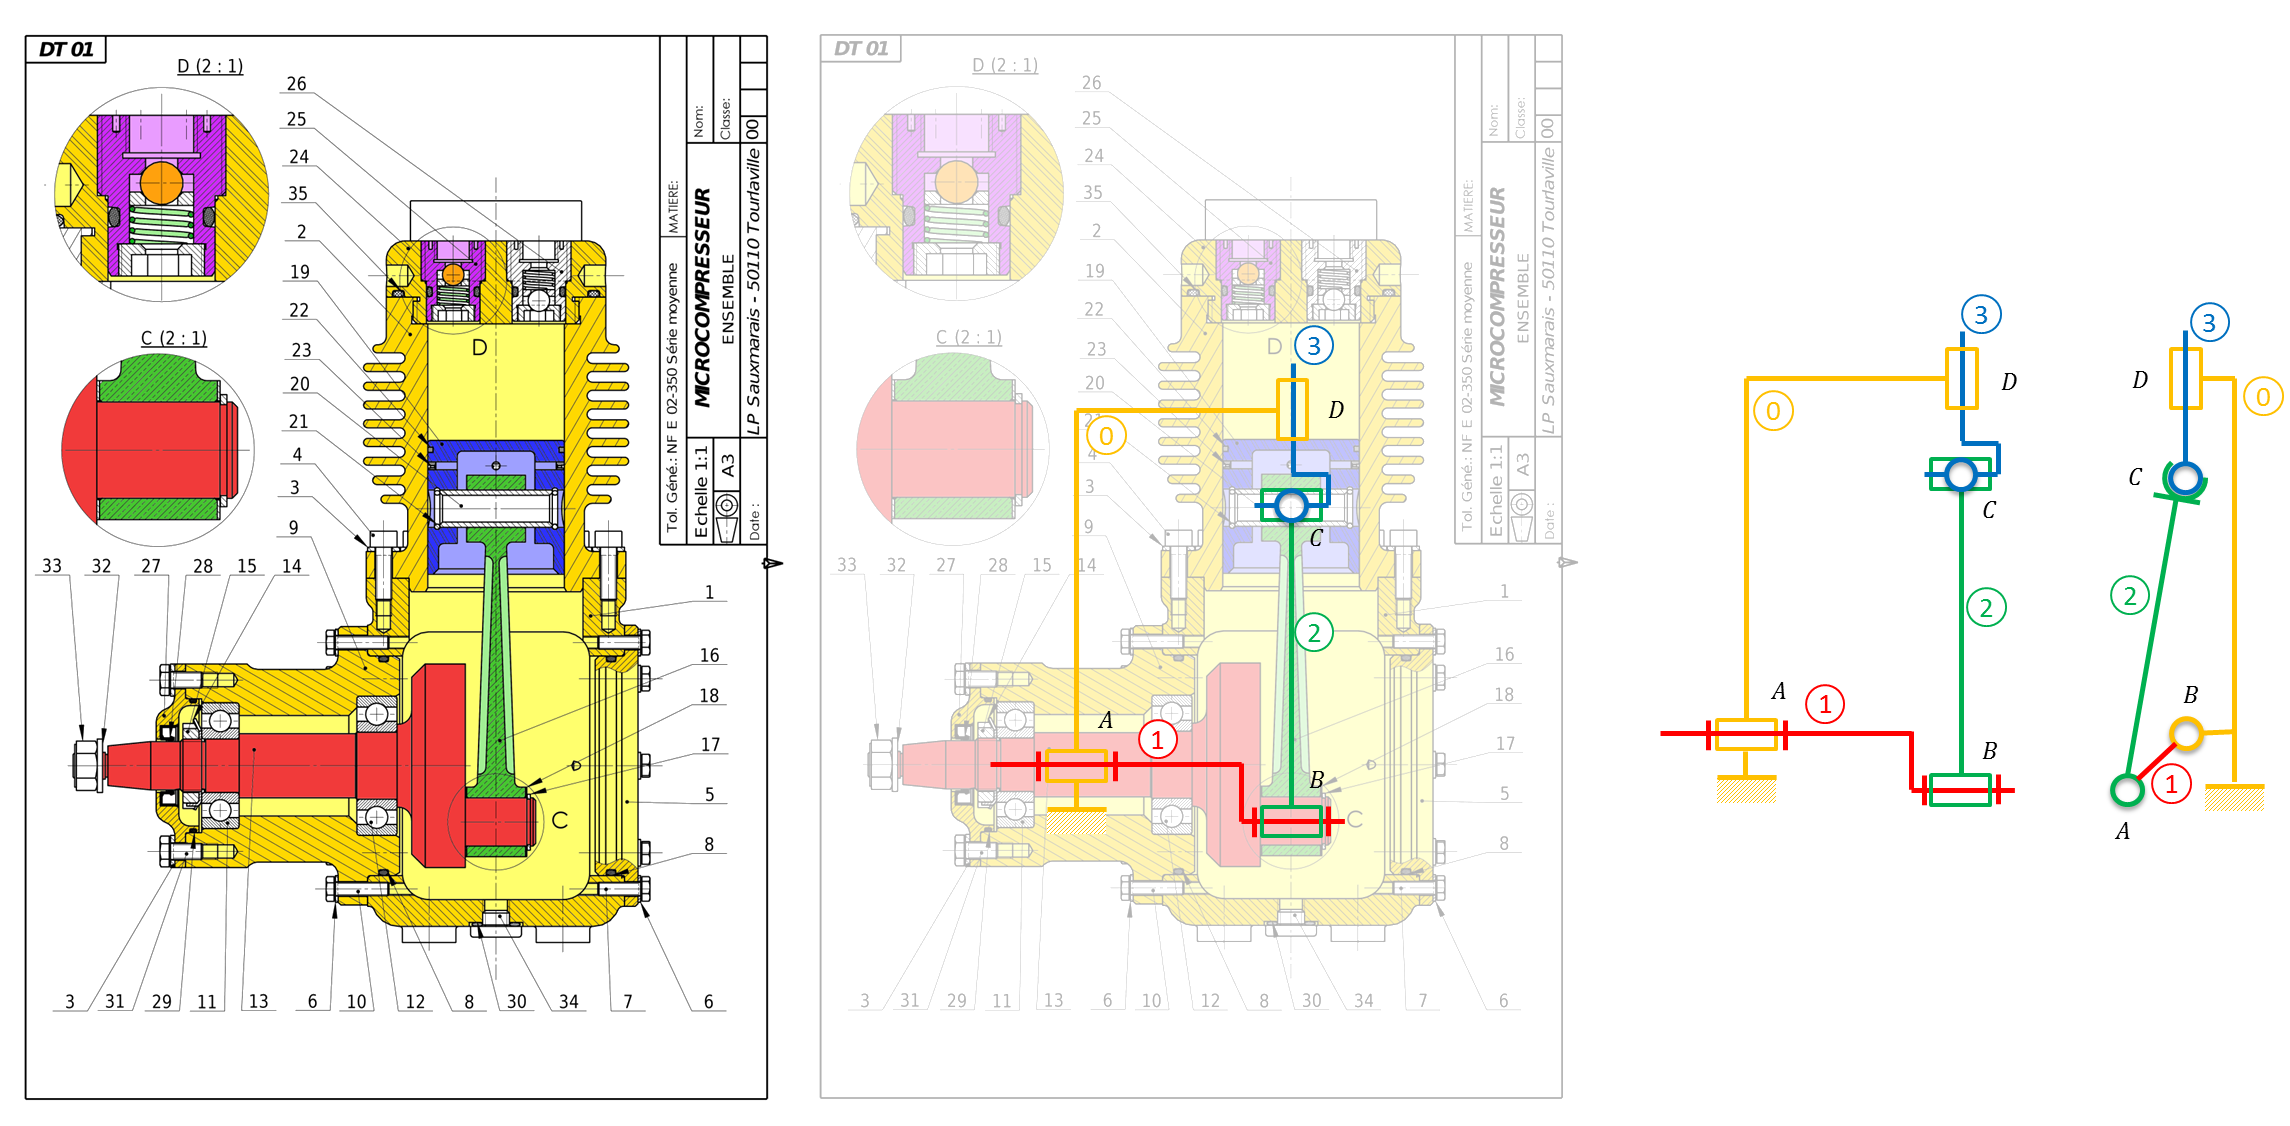
\includegraphics[width=\textwidth]{png/modelisme}
\end{center}



\begin{minipage}[c]{.6\linewidth}
\begin{center}
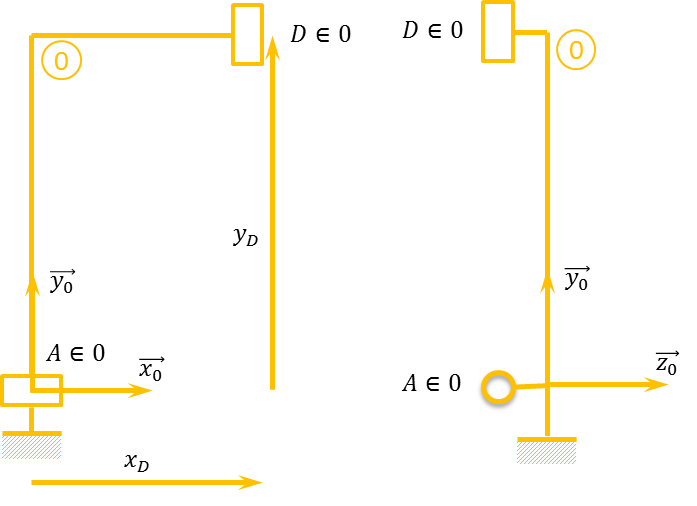
\includegraphics[width=\textwidth]{png/piece_0}
\end{center}
\end{minipage}\hfill
\begin{minipage}[c]{.3\linewidth}
En isolant le bâti 0, il est possible de lui associer un repère orthonormé $\mathcal{R}_0 \left(A,\vect{x_0},\vect{y_0},\vect{z_0}\right)$. 

On a $\vect{AD}=x_D \vect{x_0} + y_D \vect{y_0}$.

On remarque que le point $A$ appartient à la fois aux solides 0 et 1. 
\end{minipage}


\begin{minipage}[c]{.4\linewidth}
\begin{center}
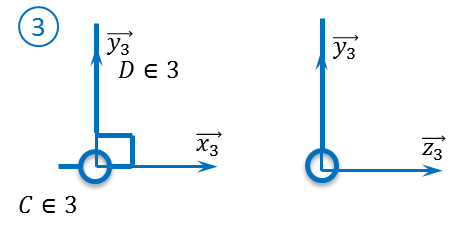
\includegraphics[width=\textwidth]{png/piece_3}

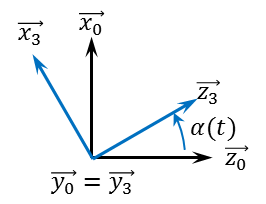
\includegraphics[width=.6\textwidth]{png/rep_3}
\end{center}
\end{minipage}\hfill
\begin{minipage}[c]{.55\linewidth}
On isole le piston 3 et on lui associe la base orthonormée directe $\mathcal{R}_3 \left(C,\vect{x_3},\vect{y_3},\vect{z_3}\right)$. 

Les pièces 0 et 3 sont en liaison pivot glissant d'axe $\vect{y_0}$. $\vect{y_0}$ et $\vect{y_3}$ ayant même direction, même sens et même norme, on a $\vect{y_0}=\vect{y_3}$.

En revanche, les pièces 0 et 3 pivotent l'une par rapport à l'autre autour de l'axe $\vect{y_0}$.

On a 
$$\alpha(t)
=\left(\widehat{\vect{z_0},\vect{z_3}}\right) 
=\left(\widehat{\vect{x_0},\vect{x_3}}\right) 
$$

Où $\alpha(t)$ est un angle en radian et $t$ est le temps en secondes. 


\end{minipage}



\subsection{Coordonnées cylindriques}

\begin{defi}
\textbf{Coordonnées polaires}

Soit $(O,\vect{i},\vect{j})$ un repère orthonormé direct du plan euclidien orienté. Pour tout $\theta \in \mathbb{R}$, on pose :
$$
\left\{
\begin{array}{l}
\vect{u}(\theta)=\cos (\theta) \vect{i} + \sin (\theta) \vect{j} \\
\vect{v}(\theta)=-\sin(\theta) \vect{i} + \cos (\theta) \vect{j}
\end{array}
\right.
$$

Le couple $(\vect{u}(\theta),\vect{v}(\theta))$ est appelé base polaire associée à l'angle $\theta$. 

Le triplet $(O,\vect{u}(\theta),\vect{v}(\theta))$ est appelé repère polaire associé à l'angle $\theta$. 

\end{defi}

\begin{defi}
\textbf{Système de coordonnées polaires}

Soit $(O,\vect{i},\vect{j})$ un repère orthonormé direct du plan euclidien orienté. 

Pour tout point $M$ du plan, on appelle systèmes de coordonnées polaires de $M$ dans $(O,\vect{i},\vect{j})$ tout couple $(r,\theta)$ de réels vérifiant $\vect{OM}=r\vect{u}(\theta)$.

\end{defi}

\begin{exemple}
\textit{Trajectoire en coordonnées polaires}

\begin{minipage}[c]{.47\linewidth}
\begin{center}
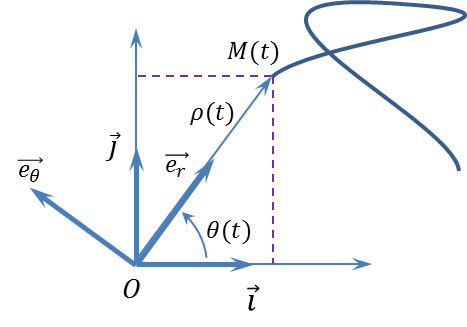
\includegraphics[width=.8\textwidth]{png/coord_polaires}
\end{center}
\end{minipage}\hfill
\begin{minipage}[c]{.47\linewidth}
Le point $M$ suit une trajectoire dans le repère $\mathcal{R}=\left(O, \vect{i},\vect{j}\right)$
$$
\vect{OM(t)}=\rho(t)\vect{e_r}=\rho(t)\cos \theta(t) \vect{i} + \rho(t)\sin \theta(t) \vect{j} 
$$
\end{minipage}

\end{exemple}

\begin{rem}
\begin{enumerate}
\item Contrairement au système de coordonnées d'un point dans un repère cartésien, les coordonnées qui viennent d'être définies ne sont pas uniques. 
\item Soit $M$ un point du plan de coordonnées cartésiennes $(x,y)$ dans $(O,\vect{i},\vect{j})$ et de coordonnées polaires $(r,\theta)$ dans ce même repère. On a alors : 
$$
\left\{
\begin{array}{l}
x = r\cos \theta \\
y = r\sin \theta
\end{array}
\right.
$$
\end{enumerate}
\end{rem}

\begin{defi}
\textbf{Coordonnées cylindriques}

Soit $(O, \vect{i}, \vect{j}, \vect{k})$ un repère orthonormé de l'espace, et $M$ un point de l'espace.

On appelle \emph{système de coordonnées cylindriques de $M$} tout triplet $(r,\theta,z)$ de réels vérifiant :
	\begin{enumerate}
	\item $z$ est la cote de $M$ dans le repère $(O, \vect{i}, \vect{j}, \vect{k})$ ;
	\item $(r,\theta)$ est un système de coordonnées polaires dans le repère $(O, \vect{i}, \vect{j})$ du projeté orthogonal de $M$ sur le plan $(xOy)$.
	\end{enumerate}
\end{defi}

\begin{exemple}
\begin{center}
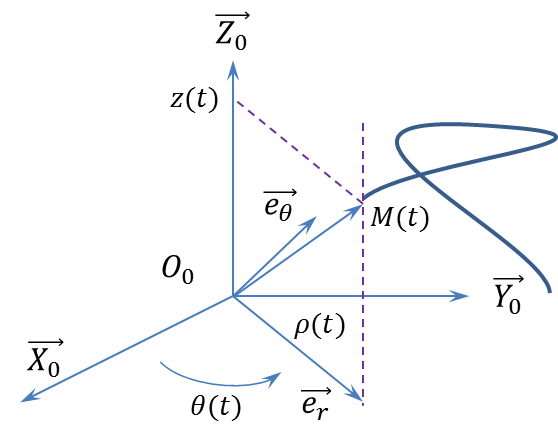
\includegraphics[width=.35\textwidth]{png/coord_cylindriques}
\end{center}
\end{exemple}

\begin{rem}
\begin{enumerate}
\item Ces coordonnées sont particulièrement adaptées pour étudier un point d'un cylindre... d'où leur nom.
\item Si le point $M$ a pour coordonnées cartésiennes $(x,y,z)$ dans $(O, \vect{i}, \vect{j}, \vect{k})$ et $(r,\theta,z)$ pour coordonnées cylindriques, alors on a :
$$\left\{
\begin{array}{l}
x=r\cos(\theta)\\
y=r\sin(\theta)
\end{array}
\right.$$
\item Comme les coordonnées polaires dans le plan, les coordonnées cylindriques ne sont pas uniques. Plus précisément, on impose l'unicité de celles-ci si on exige $r>0$ (ce qui exclut tout point de l'axe $(Oz)$) et $\theta \in ]-\pi,\pi]$, par exemple.\\
\end{enumerate}
\end{rem}


\begin{exemple}
On donne un paramétrage partiel (voir chapitre 3) du micro moteur. 
\begin{center}
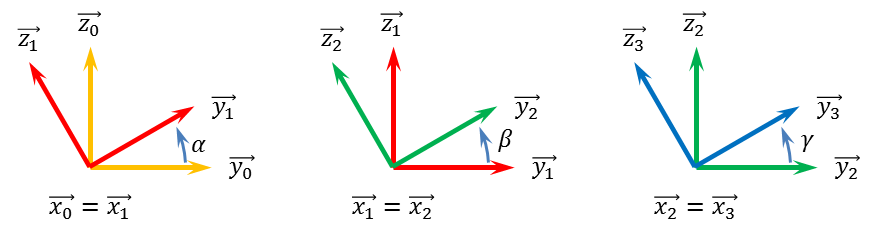
\includegraphics[width=.8\textwidth]{png/parametrage}
\end{center}
On note :
\begin{itemize}
\item $\alpha =\left(\widehat{\vect{y_0},\vect{y_1}}\right)$ l'angle permettant de passer du repère $\mathcal{R}_0$ au repère $\mathcal{R}_1$;
\item $\beta =\left(\widehat{\vect{y_1},\vect{y_2}}\right)$ l'angle permettant de passer du repère $\mathcal{R}_1$ au repère $\mathcal{R}_2$;
\item $\gamma =\left(\widehat{\vect{y_2},\vect{y_3}}\right)$ l'angle permettant de passer du repère $\mathcal{R}_2$ au repère $\mathcal{R}_3$.
\end{itemize}
Exprimer : 
\begin{itemize}
\item le vecteur $\vect{y_1}$ dans le repère $\mathcal{R}_0$;
\item le vecteur $\vect{y_2}$ dans le repère $\mathcal{R}_0$;
\item le vecteur $\vect{z_3}$ dans le repère $\mathcal{R}_0$;
\item le vecteur $\vect{z_1}$ dans le repère $\mathcal{R}_3$.
\end{itemize}
\end{exemple}



\subsection{Coordonnées sphériques}

\begin{defi}
\textbf{Coordonnées sphériques}

Soit $(O, \vect{i}, \vect{j}, \vect{k})$ un repère orthonormé de l'espace, et $M$ un point de l'espace.

On appelle \emph{système de coordonnées cylindriques de $M$} tout triplet $(r,\theta,\varphi)$ de réels vérifiant :
	\begin{enumerate}
	\item $\theta$ est une mesure dans $[0,\pi]$ de l'angle non orienté $(\vect{k}, \overrightarrow{OM})$ ;
	\item $(r\sin(\theta),\varphi)$ est un système de coordonnées polaires dans le repère $(O, \vect{i}, \vect{j})$ du projeté orthogonal de $M$ sur le plan $(xOy)$.
	\end{enumerate}
\end{defi}


\begin{exemple}
\begin{center}
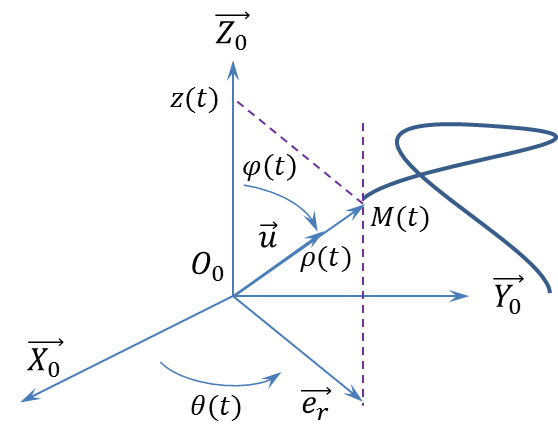
\includegraphics[width=.35\textwidth]{png/coord_spheriques}
\end{center}
\end{exemple}

\begin{rem}

\begin{enumerate}
\item Ces coordonnées sont particulièrement adaptées pour étudier un point d'une sphère. En particulier, $|r|=||\overrightarrow{OM}||$.
\item $\theta$ est appelée la \emph{colatitude}, $\varphi$ la \emph{longitude} et $\frac{\pi}{2}-\theta$ la \emph{latitude} du point $M$.
\item Si le point $M$ a pour coordonnées cartésiennes $(x,y,z)$ dans $(O, \vect{i}, \vect{j}, \vect{k})$ et $(r,\theta,\varphi)$ pour coordonnées sphériques, alors on a :
$$\left\{
\begin{array}{l}
x=r\sin(\theta)\cos(\varphi)\\
y=r\sin(\theta)\sin(\varphi)\\
z=r\cos(\theta)
\end{array}
\right.$$
\end{enumerate}
\end{rem}



%%%%%%%%%%%%%%%%%%%%%%%%%%%%


\section{Produit scalaire}
\subsection{Produit scalaire de deux vecteurs}
\begin{defi}
\textbf{Produit scalaire}

Soient $\vect{u}$ et $\vect{v}$ deux vecteurs du plan. On appelle produit scalaire de $\vect{u}$ et $\vect{v}$ et on note le réel $\vect{u}\cdot\vect{v}$ le réel : 
$$
\vect{u}\cdot\vect{v} = \left\{
\begin{array}{ll}
||\vect{u}|| \cdot ||\vect{v}|| \cdot \cos \left(\hat{\vect{u},\vect{v}}\right) & \text{ si }  \vect{u} \text{ et }  \vect{u} \text{ son non nuls } \\
0 & 
\text{ si }  \vect{u}=\vect{0} \text{ ou } \vect{v}=\vect{0}
\end{array}
\right.
$$
\end{defi}


\begin{rem}
Le résultat d'un produit scalaire est un \textbf{nombre réel}.

On a, en particulier, pour tout vecteur $\vect{u}$ du plan $\vect{u}\cdot \vect{u} = ||\vect{u}||^2$
\end{rem}

\begin{propo}
Soient $\vect{u}$ et $\vect{v}$ deux vecteurs du plan. 
$\vect{u}$ et $\vect{v}$ sont orthogonaux si et seulement si 
$\vect{u}\cdot \vect{v} = 0$
\end{propo}

\subsection{Forme bilinéaire symétrique définie positive}
\begin{propos}
\begin{enumerate}
\item Pour tout couple $(\vect{u},\vect{v})$ de vecteurs du plan $\vect{u}\cdot\vect{v} = \vect{v}\cdot\vect{u}$.
\item \begin{enumerate}
\item Pour tout triplet $(\vect{u},\vect{v_1},\vect{v_2})$ de vecteurs du plan, et pour tout couple $(\lambda,\mu)$ de réels on a : 
$$
\vect{u}\cdot\left(\lambda \vect{v_1} + \mu \vect{v_2} \right) = \lambda \vect{u}\cdot \vect{v_1} +  \mu \vect{u}\cdot \vect{v_2}
$$
\item Pour tout triplet $(\vect{u_1},\vect{u_2},\vect{v})$ de vecteurs du plan, et pour tout couple $(\lambda,\mu)$ de réels on a : 
$$
\left(\lambda \vect{u_1} + \mu \vect{u_2} \right) \cdot \vect{v}= \lambda \vect{u_1}\cdot \vect{v} +  \mu \vect{u_2}\cdot \vect{v}
$$
\end{enumerate}
\item Pour tout vecteur $\vect{u}$ du plan, $\vect{u}\cdot \vect{u}\geq 0$, et, de plus, $\vect{u}\cdot\vect{u}=0$ si et seulement si $\vect{u}=\vect{0}$.
\end{enumerate}
\end{propos}


\subsection{Expression du produit scalaire de deux vecteurs en base orthonormée}

\begin{propo}

Soient $(O, \vect{i}, \vect{j}, \vect{k})$ un repère orthonormé de l'espace, $\vect{u}$ et $\vect{v}$ deux vecteurs de l'espace, et $(x,y,z)$ et $(x',y',z')$ leurs coordonnées respectives dans $(\vect{i}, \vect{j}, \vect{k})$.

Alors :
$$\vect{u}\cdot \vect{v}=xx'+yy'+zz'$$
\end{propo}



\begin{coro}

Soient $(O, \vect{i}, \vect{k}, \vect{k})$ un repère orthonormé de l'espace, $\vect{u}$ un vecteur de l'espace, $A$ et $B$ deux points de l'espace, de coordonnées respectives $(x,y,z)$, $(x_A,y_A,z_A)$ et $(x_B,y_B,z_B)$ dans $(O, \vect{i}, \vect{j}, \vect{k})$.

Alors on a :
$$||\vect{u}||=\sqrt{x^2+y^2+z^2}  \text{ et } AB=\sqrt{(x_B-x_A)^2+(y_B-y_A)^2+(z_B-z_A)^2}.$$
\end{coro}

\section{Produit vectoriel}

Dans cette partie, on suppose que l'espace $\mathcal{E}$ est orienté.

\subsection{Produit vectoriel de deux vecteurs}

\begin{defi}
\textbf{Produit vectoriel de deux vecteurs}

Soient $\vect{u}$ et $\vect{v}$ deux vecteurs de l'espace $\mathcal{E}$ orienté.

On appelle produit vectoriel de $\vect{u}$ et $\vect{v}$ le vecteur de l'espace, noté $\vect{u} \wedge \vect{v}$, et défini par :
$$\vect{u}\wedge \vect{v}=\left\{
\begin{array}{cl}
||\vect{u}||\cdot ||\vect{v}|| \cdot \sin\left(\widehat{\vect{u}, \vect{v}}\right)\cdot\vect{k} & \text{si } \vect{u} \text{ et } \vect{v} \text{ne sont pas colinéaires}\\
\vect{0} & \text{sinon}
\end{array}
\right.$$

où $\vect{k}$ est un vecteur de norme 1, perpendiculaire au(x) plan(s) défini(s) par $\vect{u}$ et $\vect{v}$ et tel que $(\vect{u},\vect{v}, \vect{k})$ forme une base directe de l'espace.

\end{defi}

\begin{rem}
Le résultat du produit vectoriel est un \textbf{vecteur}. Comme tout vecteur il est caractérisé par :
\begin{itemize}
\item son sens : dans le sens de $\vect{k}$;
\item sa direction : direction de $\vect{k}$;
\item sa norme : $||\vect{u}||\cdot ||\vect{v}|| \cdot \sin\left(\widehat{\vect{u}, \vect{v}}\right)$
\end{itemize}
\end{rem}








\begin{propo}

Soient $\vect{u}$ et $\vect{v}$ deux vecteurs de l'espace.
\begin{enumerate}
\item $\vect{u}$ et $\vect{v}$ sont colinéaires si et seulement si $\vect{u}\wedge \vect{v}=\vect{0}$ ;
\item Si $\vect{u}$ et $\vect{v}$ ne sont pas colinéaires, alors $(\vect{u}, \vect{v}, \vect{u}\wedge\vect{v})$ est une base directe de l'espace.
\end{enumerate}
\end{propo}

\begin{rem}
En particulier, si $(\vect{i}, \vect{j}, \vect{k})$ est une base orthonormée directe de l'espace, alors $\vect{i}\wedge\vect{j}=\vect{k}$, $\vect{j} \wedge \vect{k}=\vect{i}$ et $\vect{k}\wedge \vect{i}=\vect{j}$.\\

\end{rem}



\subsection{Le produit vectoriel est bilinéaire et anti-symétrique}

\begin{propo}

\begin{enumerate}
\item Pour tout couple $(\vect{u}, \vect{v})$ de vecteurs de l'espace, $\vect{v}\wedge \vect{u}=-\left(\vect{u}\wedge\vect{v}\right)$.
\item \begin{enumerate}
	\item Pour tout triplet $(\vect{u}, \vect{v}_1, \vect{v}_2)$ de vecteurs de l'espace, et pour tout couple $(\lambda, \mu)$ de réels, on a : $$\vect{u}\wedge(\lambda \vect{v}_1+\mu \vect{v}_2)=\lambda (\vect{u}\wedge\vect{v}_1)+\mu (\vect{u}\wedge\vect{v}_2).$$
	\item Pour tout triplet $(\vect{u}_1, \vect{u}_2, \vect{v})$ de vecteurs de l'espace, et pour tout couple $(\lambda, \mu)$ de réels, on a : $$(\lambda \vect{u}_1+\mu \vect{u}_2)\wedge\vect{v}=\lambda \left(\vect{u}_1\wedge\vect{v}\right)+\mu \left(\vect{u}_2\wedge\vect{v}\right).$$
	\end{enumerate}
\end{enumerate}
\end{propo}




\subsection{Expression du produit vectoriel de deux vecteurs en base orthonormée directe}

\begin{propo}
Soient $(O, \vect{i}, \vect{j}, \vect{k})$ un repère orthonormé direct de l'espace, $\vect{u}$ et $\vect{v}$ deux vecteurs de l'espace, et $(x,y,z)$ et $(x',y',z')$ leurs coordonnées respectives dans $(\vect{i}, \vect{j}, \vect{k})$.

Alors les coordonnées de $\vect{u}\wedge\vect{v}$ dans $(\vect{i}, \vect{j}, \vect{k})$ sont  :
$$(yz'-zy',zx'-xz',xy'-x'y).$$
\end{propo}



\begin{methode}
\textbf{Calcul du produit vectoriel -- Méthode analytique}

Soient $\vect{v_1}$ et $\vect{v_2}$ deux vecteurs exprimés dans $\mathcal{R}_0$. 

On a alors :
$$
||\vect{v_1} \wedge \vect{v_2}|| = ||\vect{v_1}|| \cdot ||\vect{v_2}|| \cdot \sin \left(\vect{v_1};\vect{v_2} \right) 
$$

Le vecteur résultant du produit vectoriel de ces deux vecteurs est orthogonal au plan formé par $\vect{v_1}$ et $\vect{v_2}$. $\vect{v_1}$, $\vect{v_2}$ et le vecteur résultant doivent former un trièdre direct. 

On a :
$$
\vect{v_1} \wedge \vect{v_2} 
= 
\left[
\begin{array}{c}
v_{1x}\\
v_{1y}\\
v_{1z}\\
\end{array}
\right]_{\mathcal{R}_0}
\wedge
\left[
\begin{array}{c}
v_{2x}\\
v_{2y}\\
v_{2z}\\
\end{array}
\right]_{\mathcal{R}_0}
=
\left[
\begin{array}{c}
v_{1y}v_{2z}-v_{1z}v_{2y}\\
-\left( v_{1x}v_{2z}-v_{1z}v_{2x}\right)\\
v_{1x}v_{2y}-v_{1y}v_{2x}\\
\end{array}
\right]_{\mathcal{R}_0}
$$


\begin{minipage}[c]{.15\linewidth}
\begin{center}

\includegraphics[width=.8\textwidth]{png/warning3}
\end{center}
\end{minipage} \hfill
\begin{minipage}[c]{.8\linewidth}
Pour réaliser le produit vectoriel, les vecteurs doivent être exprimés dans le même repère.
\end{minipage}
\end{methode}

\begin{methode}
\textbf{Calcul du produit vectoriel -- Méthode graphique}

Cette méthode sera utilisée lors du produit vectoriel entre vecteurs normés. Le calcul du produit vectoriel est alors déduit de la lecture des figures planes : 

\begin{minipage}[c]{.3\linewidth}
\begin{center}
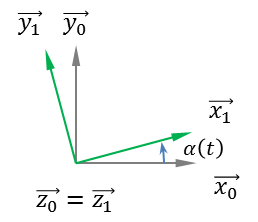
\includegraphics[width=.9\textwidth]{png/alpha}
\end{center}
\end{minipage} \hfill
\begin{minipage}[c]{.65\linewidth}
$$
\vect{x_0}\wedge\vect{y_0}=\vect{z_0}
$$
$$
\vect{x_0}\wedge\vect{x_1}=
\underbrace{+}_{\vect{x_0}  \text{ puis }\vect{x_1} \text{ dans le sens direct}}
\underbrace{\sin \alpha(t)}_{\text{angle entre} \vect{x_0} \text{ et }\vect{x_1}} 
\underbrace{\vect{z_0}}_{\text{Vecteur normal à } \vect{x_0} \text{ et }\vect{x_1}}
$$
$$
\vect{y_0}\wedge\vect{x_1}
=- \sin\left( \pi/2 - \alpha(t)\right) \vect{z_0}
=- \cos \alpha(t) \vect{z_0}
$$
\end{minipage}

\end{methode}

\begin{exemple}
On donne un paramétrage partiel (voir chapitre 3) du micro moteur. 
\begin{center}
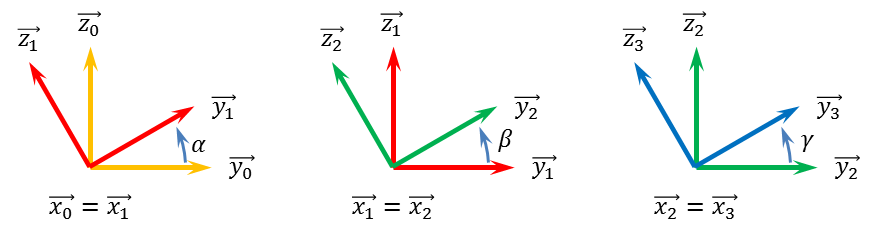
\includegraphics[width=.8\textwidth]{png/parametrage}
\end{center}
Calculer les produits vectoriels suivants : 
\begin{itemize}
\item $\vect{x_0}\wedge \vect{y_0}$;
\item $\vect{y_0}\wedge \vect{y_1}$;
\item $\vect{z_1}\wedge \vect{y_0}$;
\item $\vect{x_0}\wedge \vect{y_2}$;
\item $\vect{y_2}\wedge \vect{y_1}$;
\item $\vect{y_3}\wedge \vect{y_1}$.
\end{itemize}
\end{exemple}

%\begin{rem}
%On voit ainsi que les coordonnées de $\vect{u}\wedge \vect{v}$ sont :
%$$\left(\left|
%\begin{array}{cc}
%y & y'\\
%z & z'
%\end{array}
%\right|\, , \, \left|
%\begin{array}{cc}
%z & z'\\
%x & x'
%\end{array}
%\right|\, , \, 
%\left|
%\begin{array}{cc}
%x & x'\\
%y & y'
%\end{array}
%\right|\right).$$
%
%\end{rem}


\subsection{Double produit vectoriel}

\begin{warn}
Le produit vectoriel n'est pas associatif.

Par exemple, si $(\vect{i}, \vect{j}, \vect{k})$ est une base orthonormée directe de l'espace, alors :
$$\vect{i}\wedge \left(\vect{i} \wedge \vect{j}\right)=\vect{i}\wedge \vect{k}=-\vect{j}\  \text{ alors que }\ \left(\vect{i}\wedge\vect{i}\right)\wedge\vect{j}=\vect{0}\wedge\vect{j}=\vect{0}.$$

Il n'est donc pas licite d'écrire sans parenthèse \og{}$\vect{u}\wedge\vect{v}\wedge\vect{w}$\fg{}.\\

\end{warn}

\begin{propo}

Soient $\vect{u}$, $\vect{v}$ et $\vect{w}$ trois vecteurs de l'espace.

Alors $\vect{u} \wedge\left(\vect{v}\wedge \vect{w}\right)=\left(\vect{u} \cdot \vect{w} \right)\vect{v}-\left(\vect{u}\cdot \vect{v}\right) \vect{w}$.\\
\end{propo}


\section{Produit mixte}

Dans cette partie, on suppose que l'espace $\mathcal{E}$ est orienté.

\subsection{Produit mixte de trois vecteurs}

\begin{defi}
\textbf{Déterminant de trois vecteurs}

Soient $\vect{u}$, $\vect{v}$ et $\vect{w}$ trois vecteurs de l'espace.

On appelle produit mixte de $\vect{u}$, $\vect{v}$ et $\vect{w}$ (ou déterminant) le nombre réel défini par :
$$\Det(\vect{u}, \vect{v}, \vect{w})=\left(\vect{u}\wedge\vect{v}\right)\cdot\vect {w}$$
\end{defi}


\begin{rem}

\begin{enumerate}
\item Si l'un au moins des trois vecteurs $\vect{u}$, $\vect{v}$ et $\vect{w}$ est nul, alors $\Det(\vect{u}, \vect{v}, \vect{w})=0$.
\item Si $(\vect{i}, \vect{j}, \vect{k})$ est une base orthonormée directe, alors $\Det(\vect{i}, \vect{j}, \vect{k})=\vect{k}.\vect{k}=1$, tandis que si elle est rétrograde, $\Det(\vect{i}, \vect{j}, \vect{k})=(-\vect{k}).\vect{k}=-1$.\\
\end{enumerate}

\end{rem}
\begin{propo}

Soient $\vect{u}$, $\vect{v}$ et $\vect{w}$ trois vecteurs non nuls de l'espace.

$\vect{u}$, $\vect{v}$ et $\vect{w}$ sont coplanaires si et seulement si $\Det(\vect{u}, \vect{v}, \vect{w})=0$.
\end{propo}


\begin{rem}

\begin{enumerate}
\item En particulier, pour tout couple $(\vect{u}, \vect{v})$ de vecteurs de l'espace, $\Det(\vect{u}, \vect{u}, \vect{v})=0$ (et aussi $\Det(\vect{u}, \vect{v}, \vect{u})=0$ et $\Det(\vect{v}, \vect{u}, \vect{u})=0$).

En outre, dès que deux des trois vecteurs $\vect{u}$, $\vect{v}$ et $\vect{w}$ sont colinéaires, $\Det(\vect{u},\vect{v}, \vect{v})=0$.
\item La propriété ci-dessus permet de caractériser les bases de l'espace : étant donnés trois vecteurs $\vect{u}$, $\vect{v}$ et $\vect{w}$ de l'espace, $(\vect{u}, \vect{v}, \vect{w})$ est une base de l'ensemble des vecteurs de l'espace si et seulement si $\Det\left(\vect{u}, \vect{v}, \vect{w}\right) \neq 0$, et, plus précisément :
	\begin{itemize}\renewcommand{\labelitemi}{$\bullet$}
	\item $(\vect{u}, \vect{v}, \vect{w})$ est une base directe si et seulement si $\Det\left(\vect{u}, \vect{v}, \vect{w}\right)>0$ ;
	\item $(\vect{u}, \vect{v}, \vect{w})$ est une base indirecte si et seulement si $\Det\left(\vect{u}, \vect{v}, \vect{w}\right)<0$.\\
	\end{itemize}
\end{enumerate}
\end{rem}

\begin{rem}
\textbf{Interprétation en termes de volume}

Soient $\vect{u}$, $\vect{v}$ et $\vect{w}$ trois vecteurs non coplanaires de l'espace.
$|\Det(\vect{u}, \vect{v}, \vect{w})|$ est le volume du parallélépipède construit sur $\vect{u}$, $\vect{v}$ et $\vect{w}$.\\

\end{rem}

\subsection{Le déterminant est une forme trilinéaire anti-symétrique}

\begin{propo}
%{\bf :}

Pour tout triplet $(\vect{u}, \vect{v}, \vect{w})$ de vecteurs de l'espace, on a :
$\Det(\vect{v},\vect{u}, \vect{w})=-\Det(\vect{u},\vect{v}, \vect{w})$, $\Det(\vect{u},\vect{w}, \vect{v})=-\Det(\vect{u},\vect{v}, \vect{w})$, $\Det(\vect{w},\vect{v}, \vect{u})=-\Det(\vect{u},\vect{v}, \vect{w}).$

Autrement dit, le déterminant change de signe quand on échange deux vecteurs.
\end{propo}

\begin{rem}

On dit que le déterminant est une application \emph{anti-symétrique}.
\end{rem}

\begin{coro}
Pour tout triplet $(\vect{u}, \vect{v}, \vect{w})$ de vecteurs de l'espace, on a :
$$\Det(\vect{u},\vect{v}, \vect{w})=\Det(\vect{v},\vect{w}, \vect{u})=\Det(\vect{w},\vect{u}, \vect{v}).$$

Autrement dit, le produit vectoriel est \emph{invariant par permutation circulaire}.\\
\end{coro}


\section{Champ de vecteurs}
\subsection{Définition}
\begin{defi}
\textbf{Champ de vecteur}

Un champ de vecteur est une application qui a tout point $A$ de l'espace fait correspondre un vecteur. 
\end{defi}

On représente graphiquement la valeur de ce champ au point 
$A$ (c'est-à-dire le vecteur $\vect{V_A}$) par son représentant ayant pour origine le point $A$. 

\begin{exemple}
\textit{Champ des vecteurs vitesses pour un solide en translation uniforme et pour un solide en rotation uniforme.}

\begin{center}
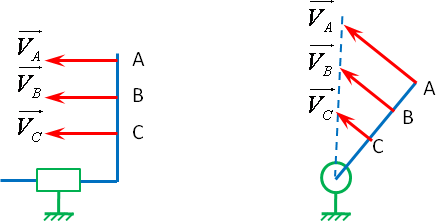
\includegraphics[width=.5\textwidth]{png/champs}
\end{center}

\end{exemple}
Un champ de vecteur peut dépendre de paramètres scalaires comme le temps par exemple. 

\subsection{Exemple de champs}

\begin{defi}
\textbf{Champ uniforme}

Les vecteurs du champ sont partout les mêmes. 

\end{defi}

\begin{defi}
\textbf{Champ équiprojectif}

Un champ est équiprojectif si quels que soient les points $A$ et $B$, on a : 
$$
\vect{AB}\cdot \vect{V_A} = \vect{AB}\cdot \vect{V_B} 
$$

\end{defi}

\begin{rem}
\begin{minipage}[c]{.47\linewidth}
On peut diviser cette relation pour faire apparaître le vecteur unitaire : $\vect{u}=\dfrac{\vect{AB}}{||\vect{AB}||}$ : 
$$
\dfrac{\vect{AB}\cdot \vect{V_A} }{||\vect{AB}||} 
=\dfrac{\vect{AB}\cdot \vect{V_B} }{||\vect{AB}||} 
\quad \text{donc} \quad
\vect{u}\cdot \vect{V_A} = \vect{u}\cdot \vect{V_B} 
$$ 
 En conséquence, $a=b$.

\end{minipage}\hfill
\begin{minipage}[c]{.47\linewidth}

\begin{center}
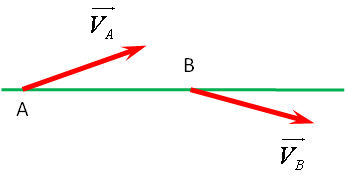
\includegraphics[width=.8\textwidth]{png/equiproj}
\end{center}
\end{minipage}
\end{rem}

\section{Moments}

\subsection{Moment en un point d'un pointeur}

\begin{defi}
\textbf{Pointeur}

On appelle pointeur $(O,\vect{V})$ l'ensemble liant un point origine $O$ est un vecteur $\vect{V}$. 
\end{defi}

\begin{defi}
\textbf{Moment en un point d'un pointeur}

\begin{minipage}[c]{.5\linewidth}
On définir le moment en un point $A$ du pointeur $(M,\vect{V})$ par : 
$$
\vect{\mathcal{M}(A,(M,\vect{V})} = \vect{AM}\wedge\vect{V}
$$

Le moment est un vecteur (résultat d'un produit vectoriel) et on choisit de le représenter graphiquement par son représentant d'origine A. 

$A$, $M$ et $\vect{V}$ appartiennent au même plan $\mathcal{P}$. 
\end{minipage}\hfill
\begin{minipage}[c]{.4\linewidth}
\begin{center}
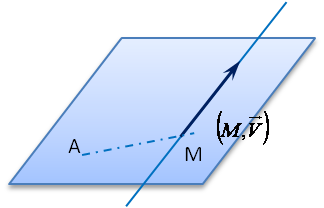
\includegraphics[width=.8\textwidth]{png/moment}
\end{center}
\end{minipage}
\end{defi}

\begin{props}
\begin{enumerate}
\item Si le point $A$ est sur le support du pointeur $(M,\vect{V})$ les vecteurs $\vect{AM}$ et $\vect{V}$ sont colinéaires et le produit vectoriel est nul; donc : 
$\vect{\mathcal{M}(A\in\text{support},(M,\vect{V})} = \vect{AM} \wedge \vect{V} =\vect{0}$.
\item Soit un point $M'$ situé sur le support du pointeur $(M,\vect{V})$ (voir figure précédente). Calculons le moment en $A$ du pointeur $(M',\vect{V})$ :
$\vect{\mathcal{M}(A,(M',\vect{V})} = \vect{AM'} \wedge \vect{V} = \left(\vect{AM}+\vect{MM'} \right)\wedge \vect{V} = \vect{AM}\wedge \vect{V}+\vect{MM'}\wedge \vect{V}$. Or $\vect{MM'}\wedge\vect{V}=\vect{0}$ car ce sont des vecteurs colinéaires. On a donc :
$\vect{\mathcal{M}(A,(M',\vect{V})} = \vect{AM}\wedge \vect{V}$.
\item On ne change pas le moment d'un pointeur lorsqu'on déplace son origine sur son support. 
\end{enumerate}
\end{props}

\begin{rem}
\textit{Relation entre les moments en deux points différents d'un même pointeur}

Calculons le moment un point $B$ du pointeur $(M,\vect{V})$. 
\end{rem}


%\subsection{Moment d'un pointeur par rapport à un axe}
%\begin{defi}
%%\begin{minipage}[c]{.47\linewidth}
%Considérons un axe $\Delta$ orienté de vecteur unitaire $\vect{u}$, un point $A$ de cet axe et le pointeur $(M,\vect{V})$. 
%
%Le moment de ce pointeur par rapport à l'axe $\Delta$ s'exprime par :
%$$
%\mathcal{M}(\Delta,(M,\vect{V}) =
%\vect{\mathcal{M}(A,(M,\vect{V})}\cdot \vect{u}
%$$
%%\end{minipage}\hfill
%%\begin{minipage}[c]{.47\linewidth}
%%\end{minipage}
%\end{defi}
%
%Le moment d'un pointeur par rapport à une droite est un scalaire positif ou négatif d'où l'importance de l'orientation de l'axe. 
%
%\begin{props}
%Exprimons ce moment en un point $B$ appartenant aussi à l'axe $\Delta$ :
%$\vect{\mathcal{M}(B,(M,\vect{V})}\cdot \vect{u} = \vect{\mathcal{M}(A,(M,\vect{V})}\cdot \vect{u} +****
%=\vect{\mathcal{M}(A,(M,\vect{V})}\cdot \vect{u} + ****$.
%
%On remarque que *****
%
%Conclusion, $\vect{\mathcal{M}(B,(M,\vect{V})}\cdot \vect{u} = ****$ avec $A$ et $B$ appartenant à $\Delta$.
%
%Ceci justifie le fait que la notation du moment d'un pointeur par rapport à un axe ne fait pas intervenir de point. 
%
%\end{props}


\begin{thebibliography}{2}
\bibitem[1]{PS} Pierrick Soleillant, Cours de Mathématiques de CPGE. Rappels de géométrie plane -- Géométrie plane élémentaire -- Géométrie dans l'espace élémentaire.
\bibitem[2]{DP} Daniel Perrin, Mathématiques d'école : Nombres, mesures et géométrie.
\bibitem[3]{cite1} Renault, \textit{Au c\oe{}ur de la technique}, \url{www.renault.com/fr/Innovation/au-coeur-de-la-technique/Pages/au-coeur-de-la-technique.aspx}.
\bibitem[4]{cite2} Wikipedia, \textit{Modélisation cinématique des mécanismes}, \url{http://fr.wikipedia.org/w/index.php?title=Mod\%C3\%A9lisation_cin\%C3\%A9matique_des_m\%C3\%A9canismes\&oldid=70679121}.
\bibitem[5]{JPP} Jean-Pierre Pupier -- Calcul vectoriel -- PTSI -- Lycée Rouvière Toulon.
\end{thebibliography}
\end{document}

